\documentclass[a4paper]{article}
\usepackage[a4paper, total={6in, 9in}]{geometry}
\usepackage[amssymb]{SIunits}
\addunit{\byte}{B}
\usepackage[nottoc,numbib]{tocbibind}
\setlength\parindent{0pt}
\usepackage[toc,page]{appendix}
\usepackage{comment}
\usepackage{listings}
\usepackage{graphicx}
\usepackage{subcaption}
\usepackage{caption}
\usepackage{tikz}
\usepackage{afterpage}
\usepackage[percent]{overpic}
\usepackage[hidelinks]{hyperref}
\lstset{
    alsoletter={()[].=},
    keywordstyle=\color{RoyalBlue},
    basicstyle=\small\ttfamily,columns=fullflexible,
    commentstyle=\color{Green}\ttfamily,
    stringstyle=\ttfamily\color{Red},
    numbers=none,
    numberstyle=\scriptsize,
    stepnumber=5,
    numbersep=8pt,
    showstringspaces=false,
    breaklines=true,
    frameround=ftff,
    frame=single,
    breakindent=5pt,
    belowcaptionskip=.75\baselineskip,
    breakatwhitespace=true,
    prebreak=\small\symbol{'134}
    %postbreak=\raisebox{0ex}[0ex][0ex]{\ensuremath{\hookrightarrow\space}}
}

\DeclareCaptionLabelFormat{subfigure}{Figure#1~\thefigure#2:}
\captionsetup[sub]{labelformat=subfigure}

\begin{document}
\author{Thomas Eichhorn\footnote{thomas.eichhorn@desy.de}~ and Jonas R\"ubenach, DESY}
\date{\today}
\title{The DESY FH E-Lab Probe Station}
\maketitle
\begin{abstract}
This document describes the operation of the probe station in the clean room of the FH E-Lab at DESY and the use of the corresponding software.
Chapter~\ref{sec:hw} lists the available hardware and how the devices should be connected.
In chapter~\ref{sec:meas} the steps needed to perform a measurement are explained together with details on how to use the measurement software.\\ \newline
The most recent versions of this manual and the software can be found at~\cite{ref:github}.
\end{abstract}

\tableofcontents

\newpage
\section{Hardware Setup}
\label{sec:hw}

This chapter gives an overview of the probe station's devices and their default connections.
After a measurement, all connections should be returned to this default state and the devices turned off.\\

\subsection{Cold Box}
\label{sec:coldbox}

The cold box case contains the probe needles and the chuck with their electrical connections.
An outside view of the cold box is shown in figure~\ref{fig:outsidecoldbox}, an inside view in figure~\ref{fig:insidecoldbox}.\\

\begin{figure}[hbtp]
\centering
\begin{subfigure}[t]{0.475\textwidth}
\centering\captionsetup{width=.8\linewidth}%
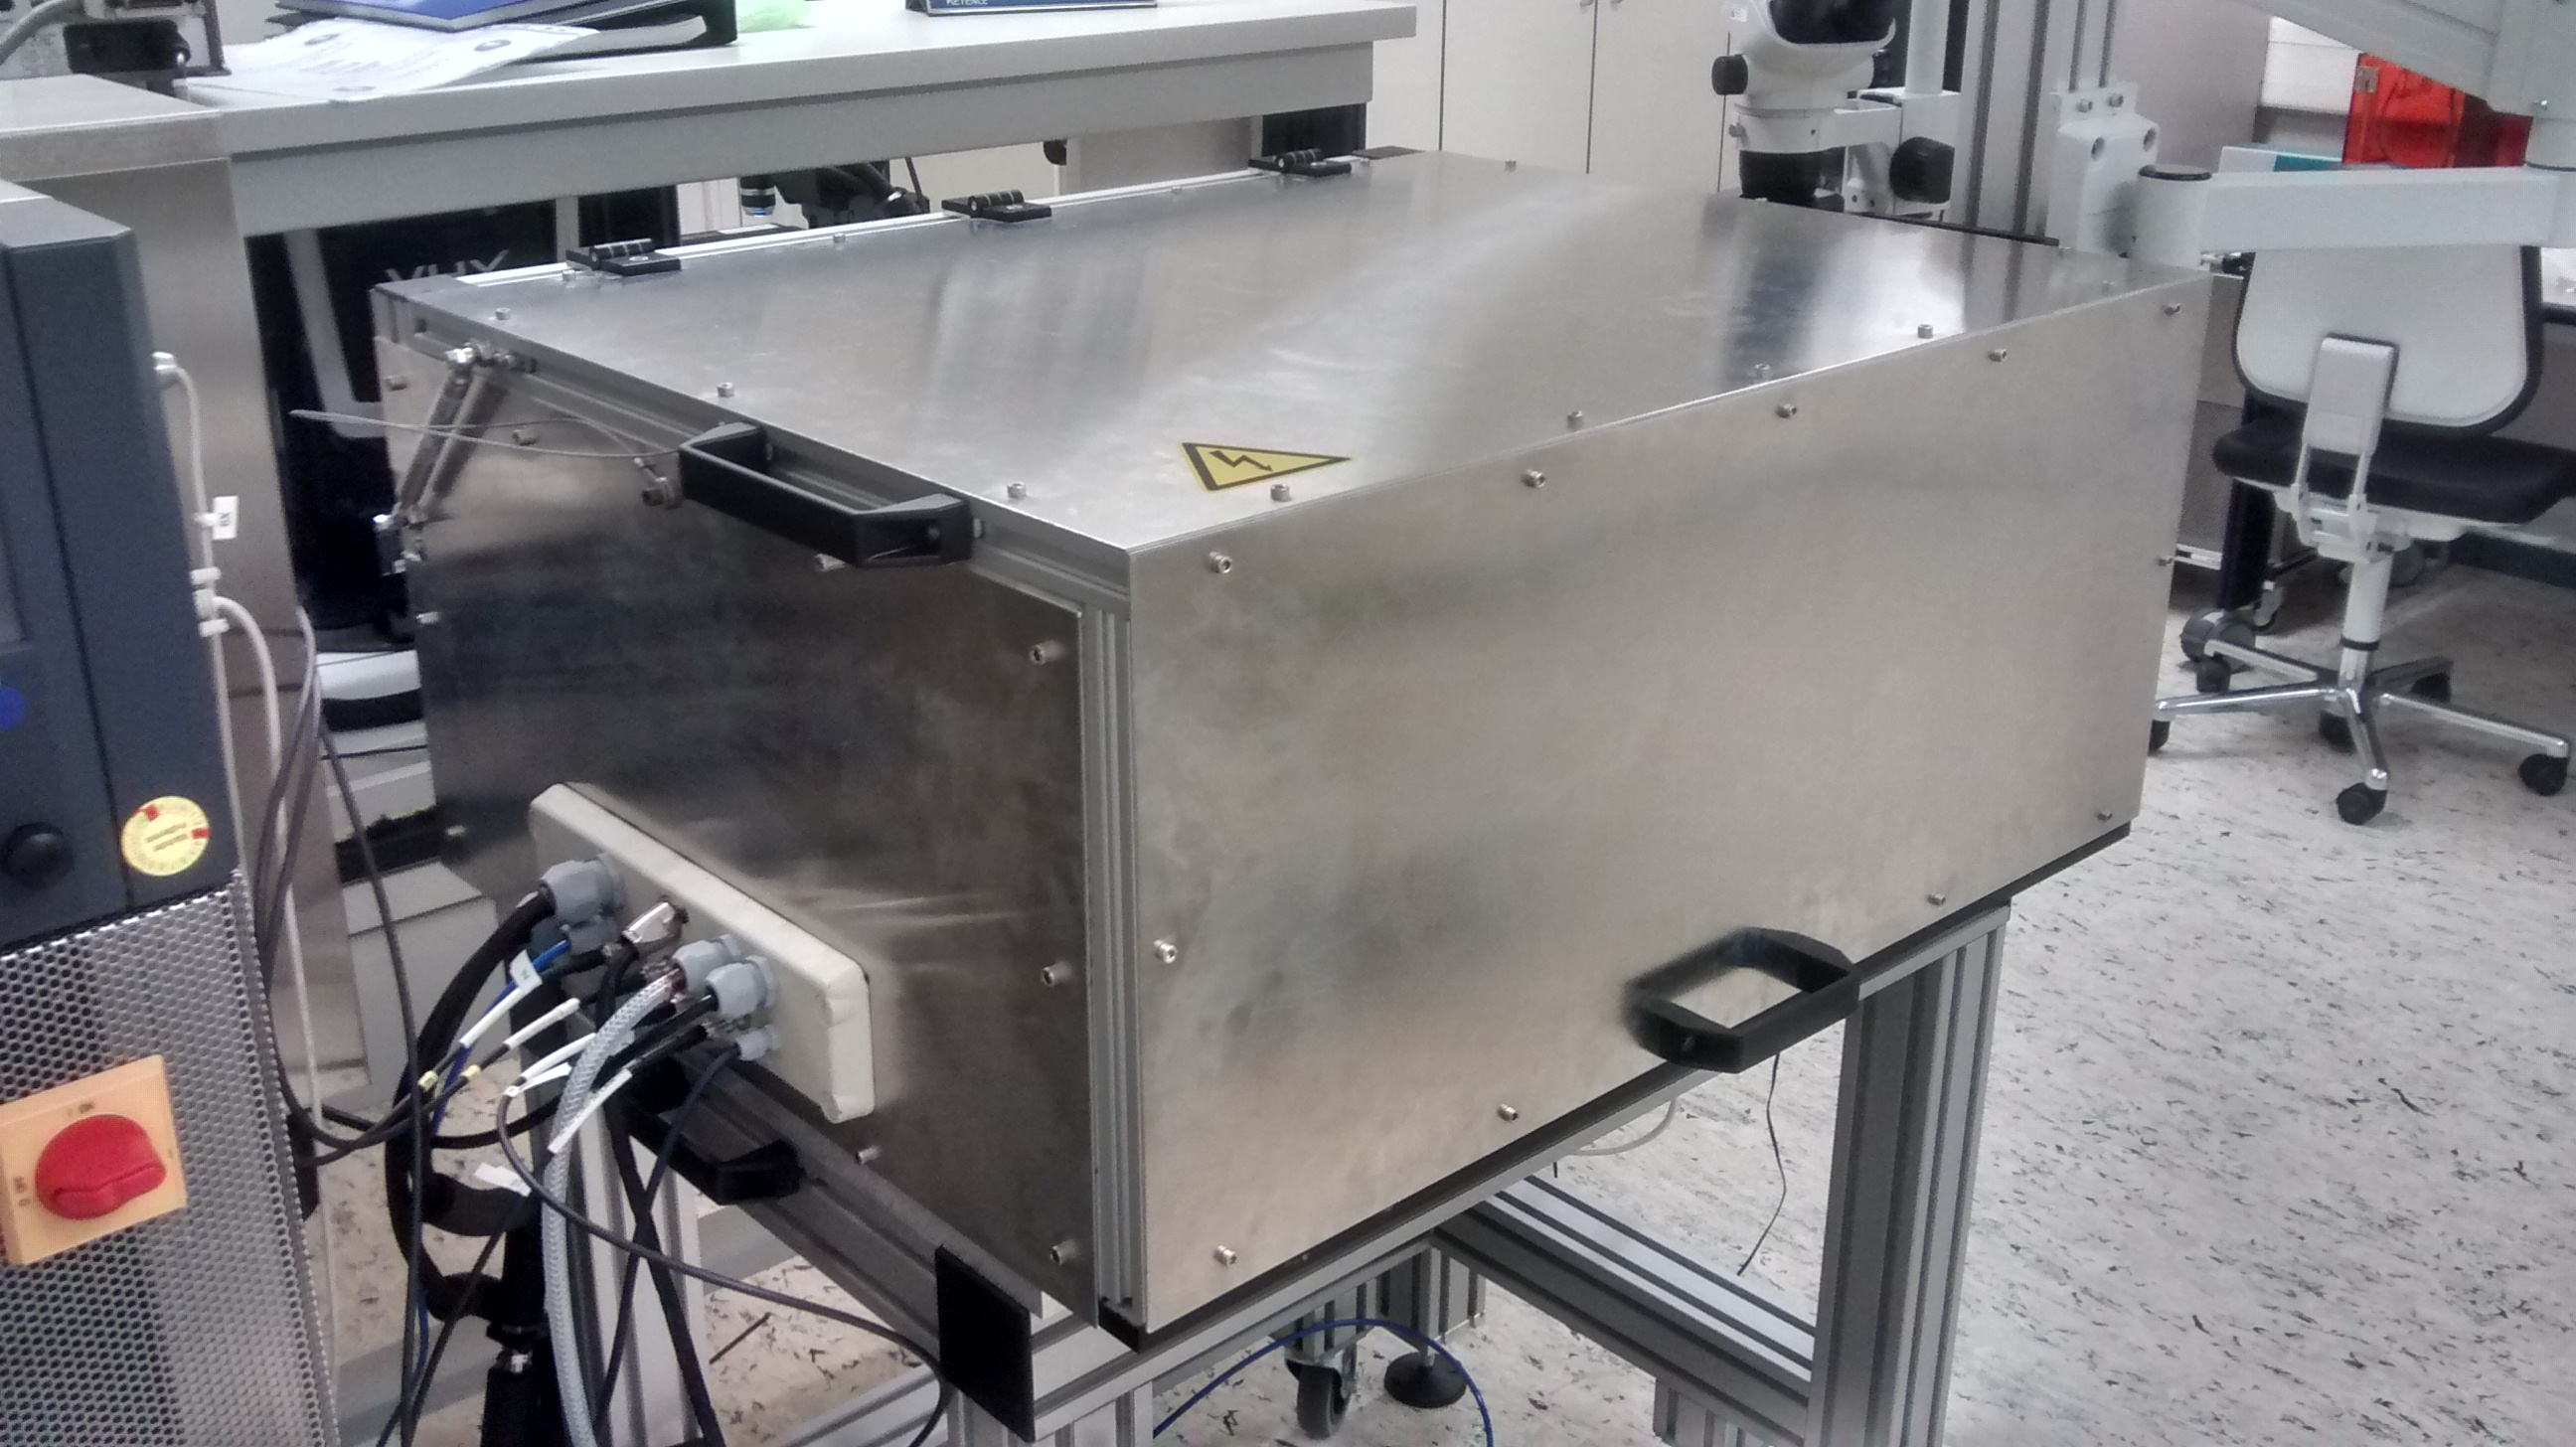
\includegraphics[width=\linewidth]{pictures/box.jpg}
\captionof{figure}[The Cold Box from the Outside]{Outside view of the cold box.}
\label{fig:outsidecoldbox}
\end{subfigure}
\begin{subfigure}[t]{0.475\textwidth}
\centering\captionsetup{width=.8\linewidth}%
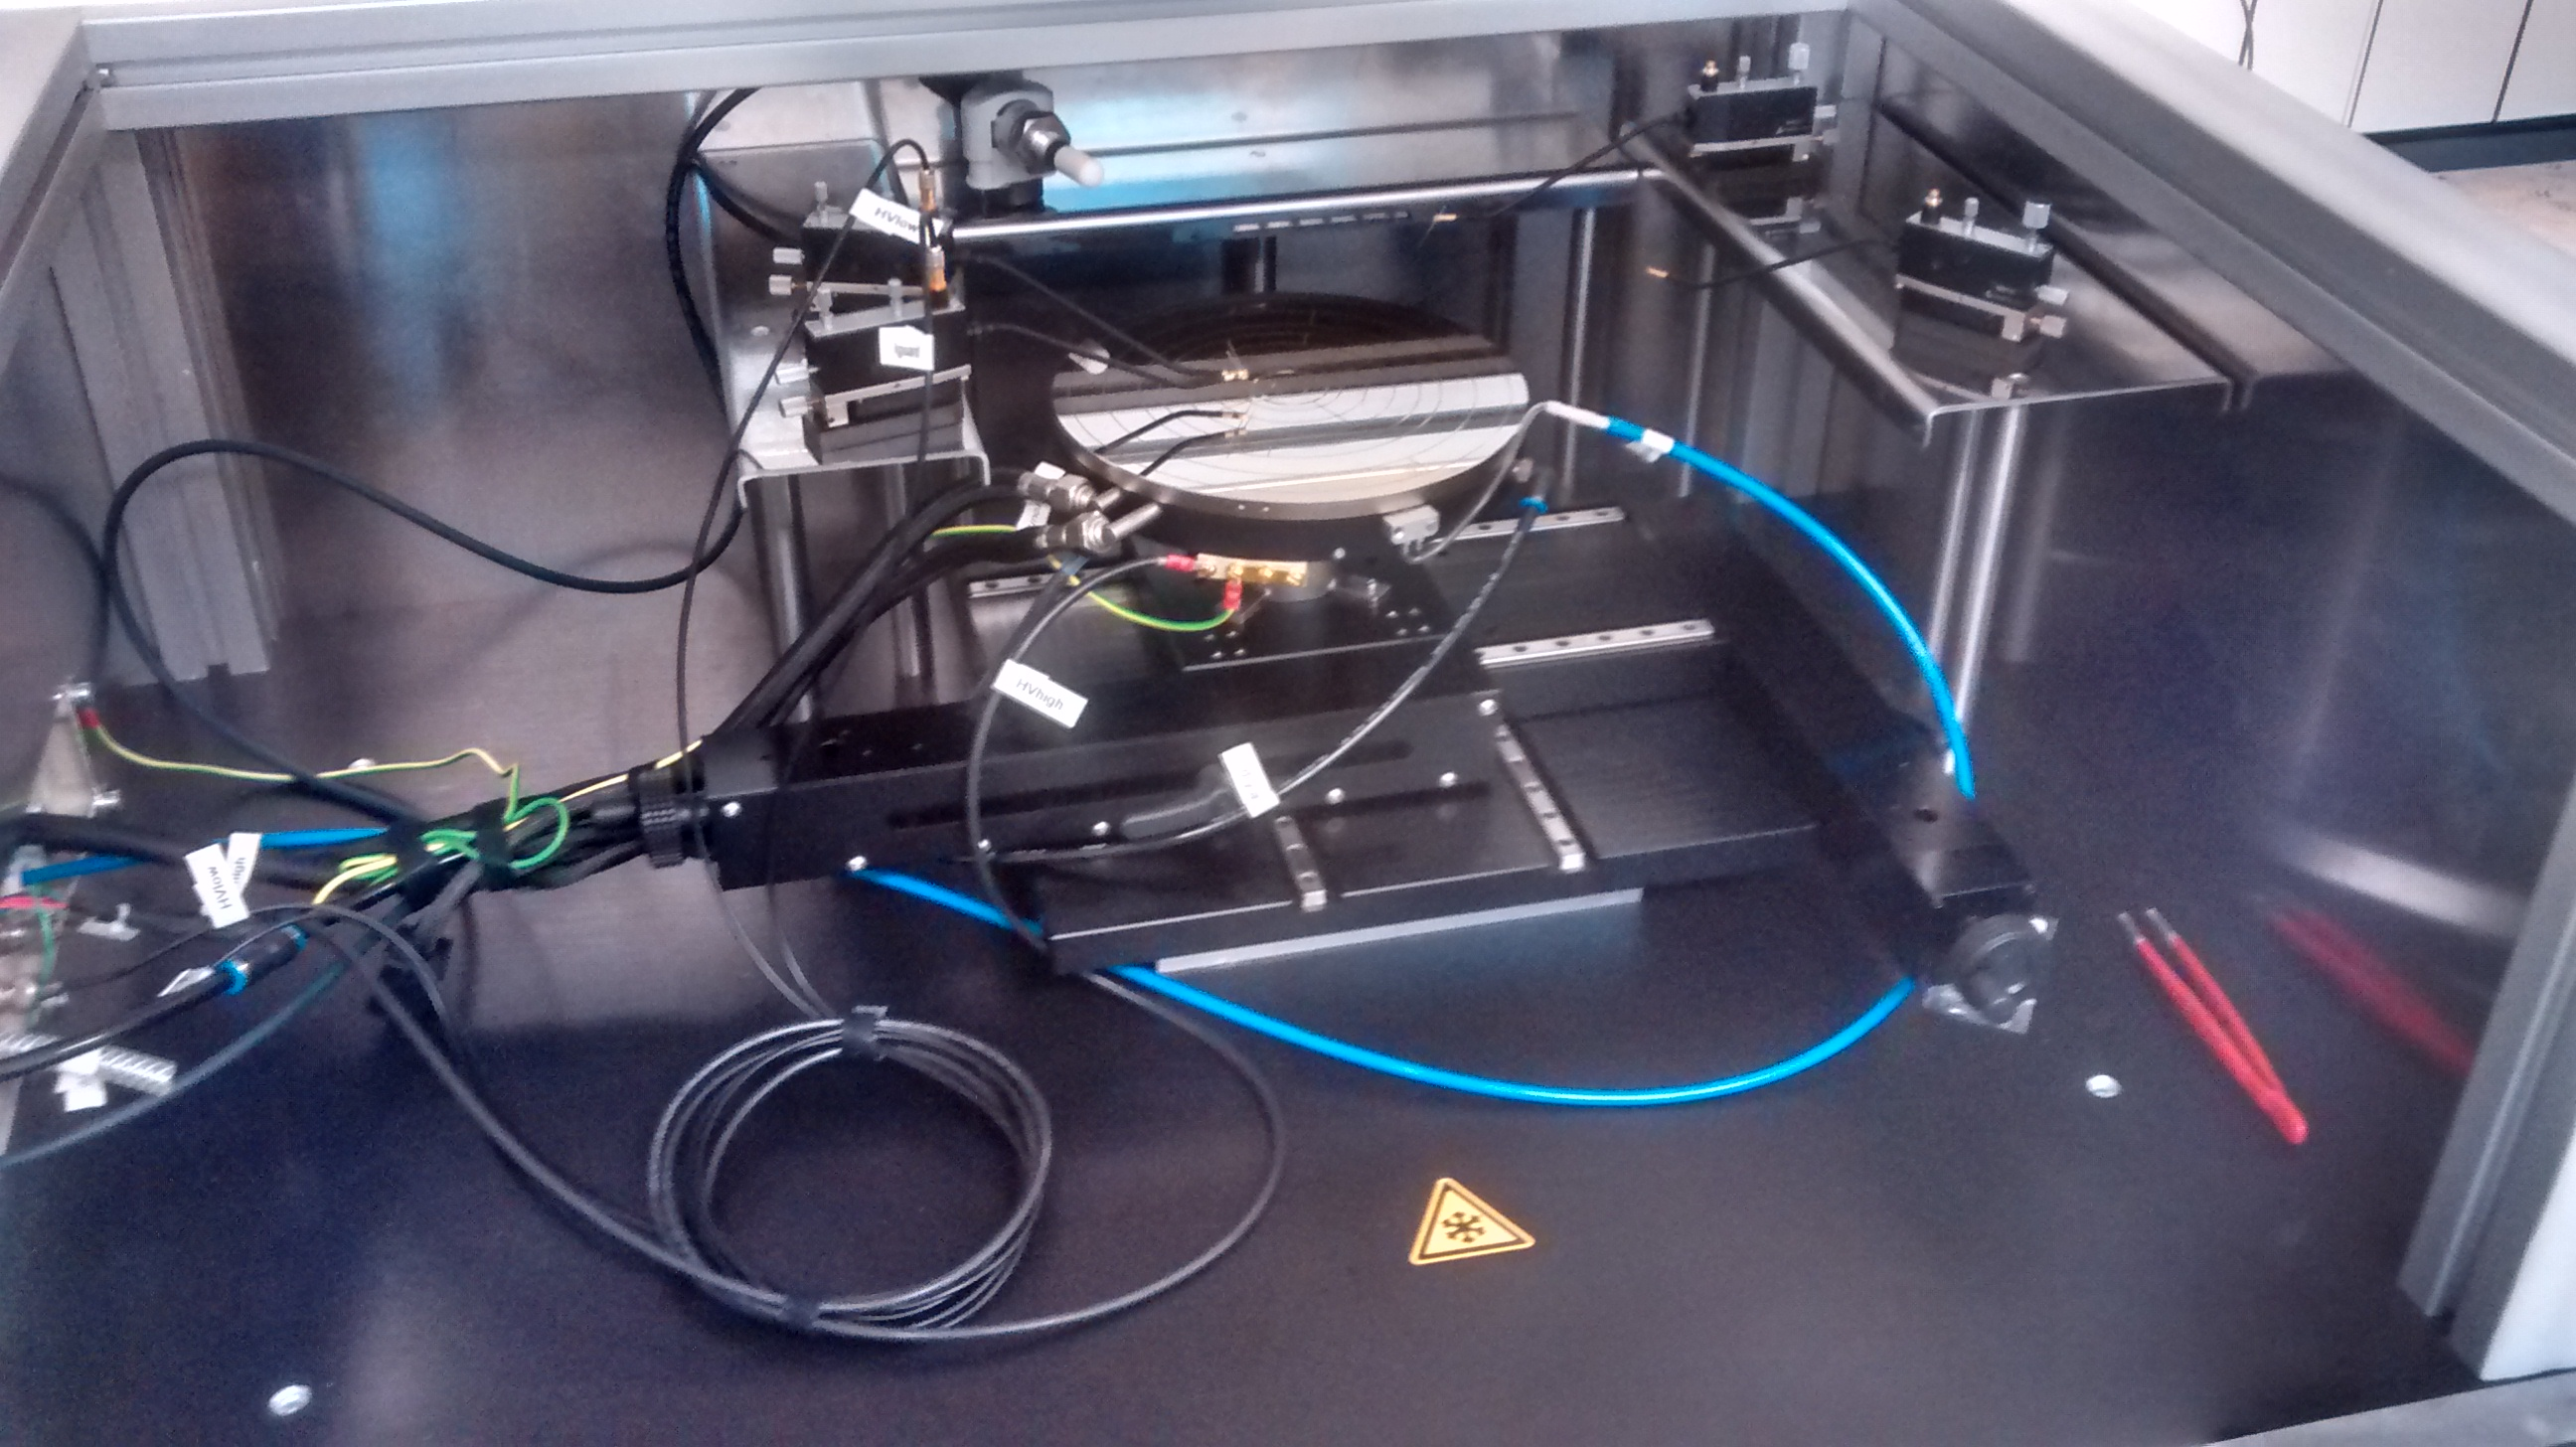
\includegraphics[width=\linewidth]{pictures/inside_box.jpg}
\captionof{figure}[The Cold Box from the Inside]{Inside view of the Cold Box with the chuck.}
\label{fig:insidecoldbox}
\end{subfigure}
\end{figure}

When opening and closing the lid of the cold box, beware not to trap any cables.
All cabling and piping should be routed via the connection panel on the lower left side of the cold box.
For safety reasons, any voltage output should be turned off before opening the lid.
This also prevents possible excess currents on the DUT ({\it device under test}) due to ambient light.

Especially for low-temperature operations, the cold box should be flushed with dry air to prevent condensation.
To activate the flow of dry air to the cold box, open the valve beneath the window of the clean room, next to the door.
The hose leading to the probe station is marked.
To change the flow of air, pull out the knob.
Turning counter-clockwise decreases the air flow, clockwise turns increase it.\\

\subsection{Microscope}
\label{sec:microscope}

The Olympus SZ61 microscope is attached to the cold box via a movable arm.
A switch on the lower part of the black lens casing turns on the light.
While moving the microscope, be careful that the light's power cable does not get trapped inside the cold box.
The microscope is used for placement of DUTs on the chuck and the positioning of the probe needles.
An example operation is shown in figure~\ref{fig:microscope}.\\

\subsection{Compressor}
\label{sec:compressor}

The compressor shown in figure~\ref{fig:compressor} is connected to the mains and to the chuck inside the cold box via a blue vacuum pipe.
The vacuum created by the compressor is used to fix DUTs on the chuck.
Currently, the outer vacuum hole on the chuck is connected.
The compressor is operated by its orange switch.\\

\begin{figure}[hbtp]
\centering
\begin{subfigure}[t]{0.475\textwidth}
\centering\captionsetup{width=.8\linewidth}%
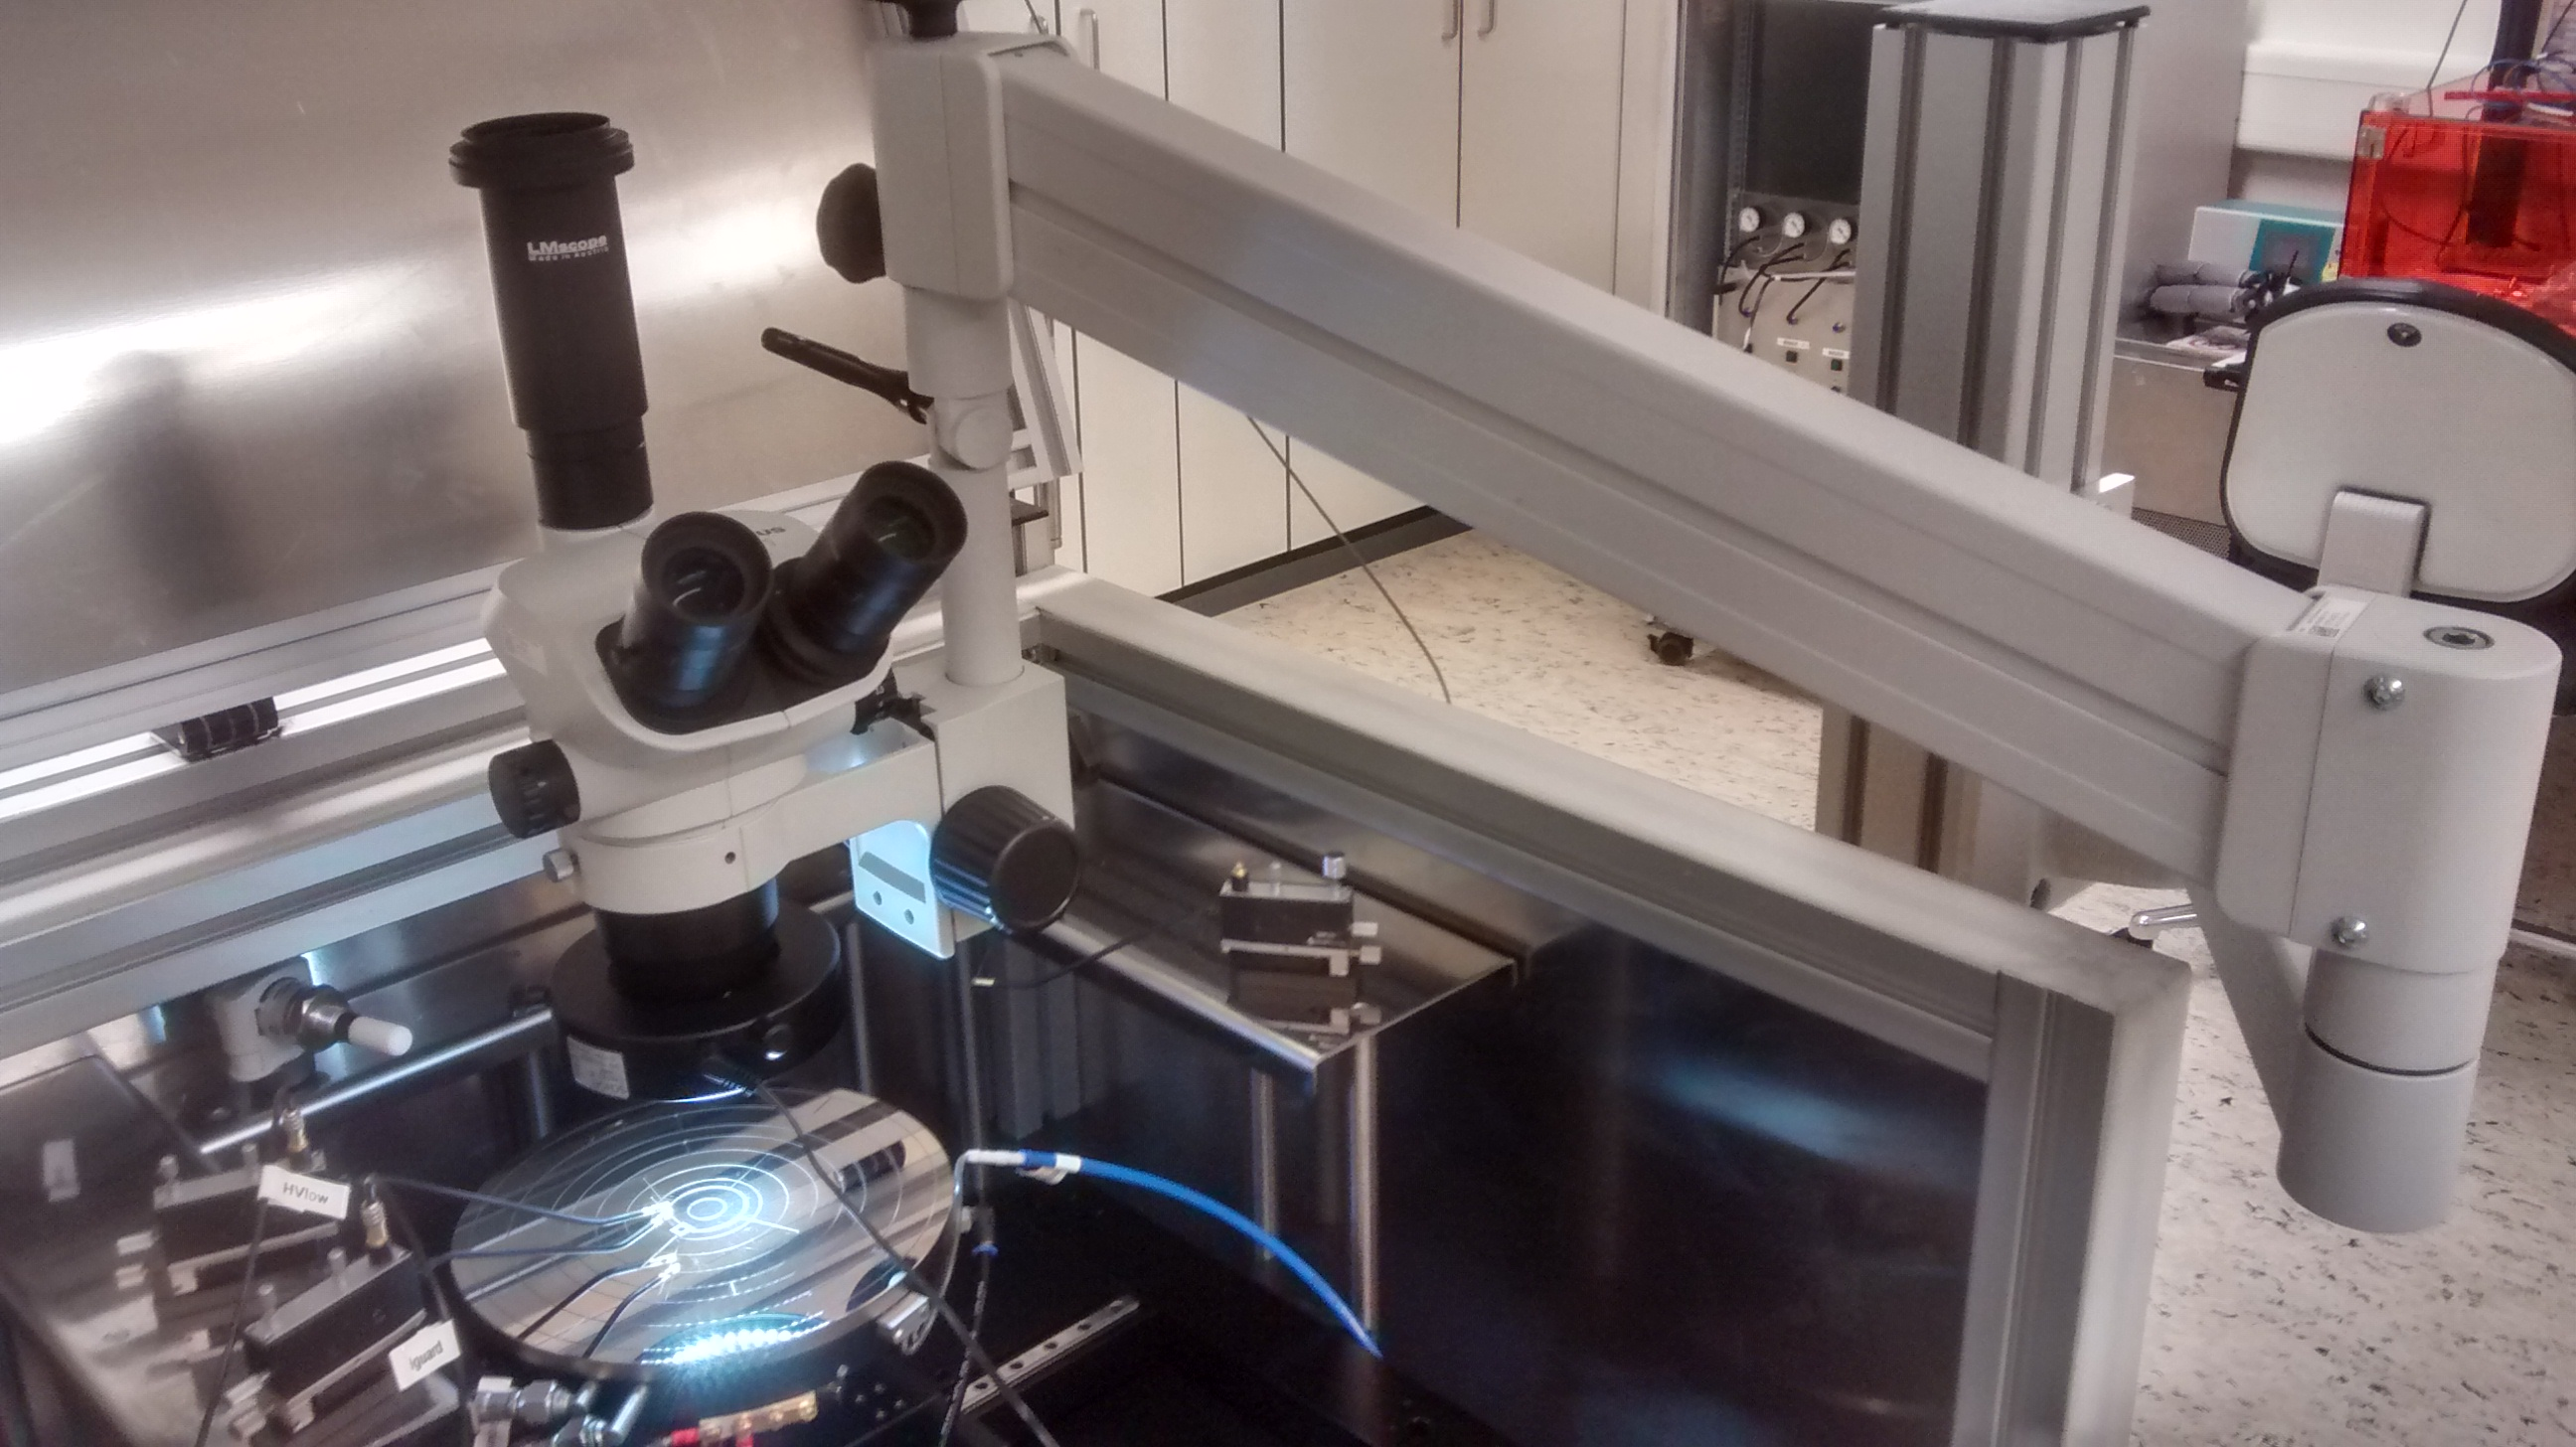
\includegraphics[width=\linewidth]{pictures/microscope.jpg}
\caption[The Microscope]{The microscope being used for positioning the needle probes.}
\label{fig:microscope}
\end{subfigure}
\begin{subfigure}[t]{0.475\textwidth}
\centering\captionsetup{width=.8\linewidth}%
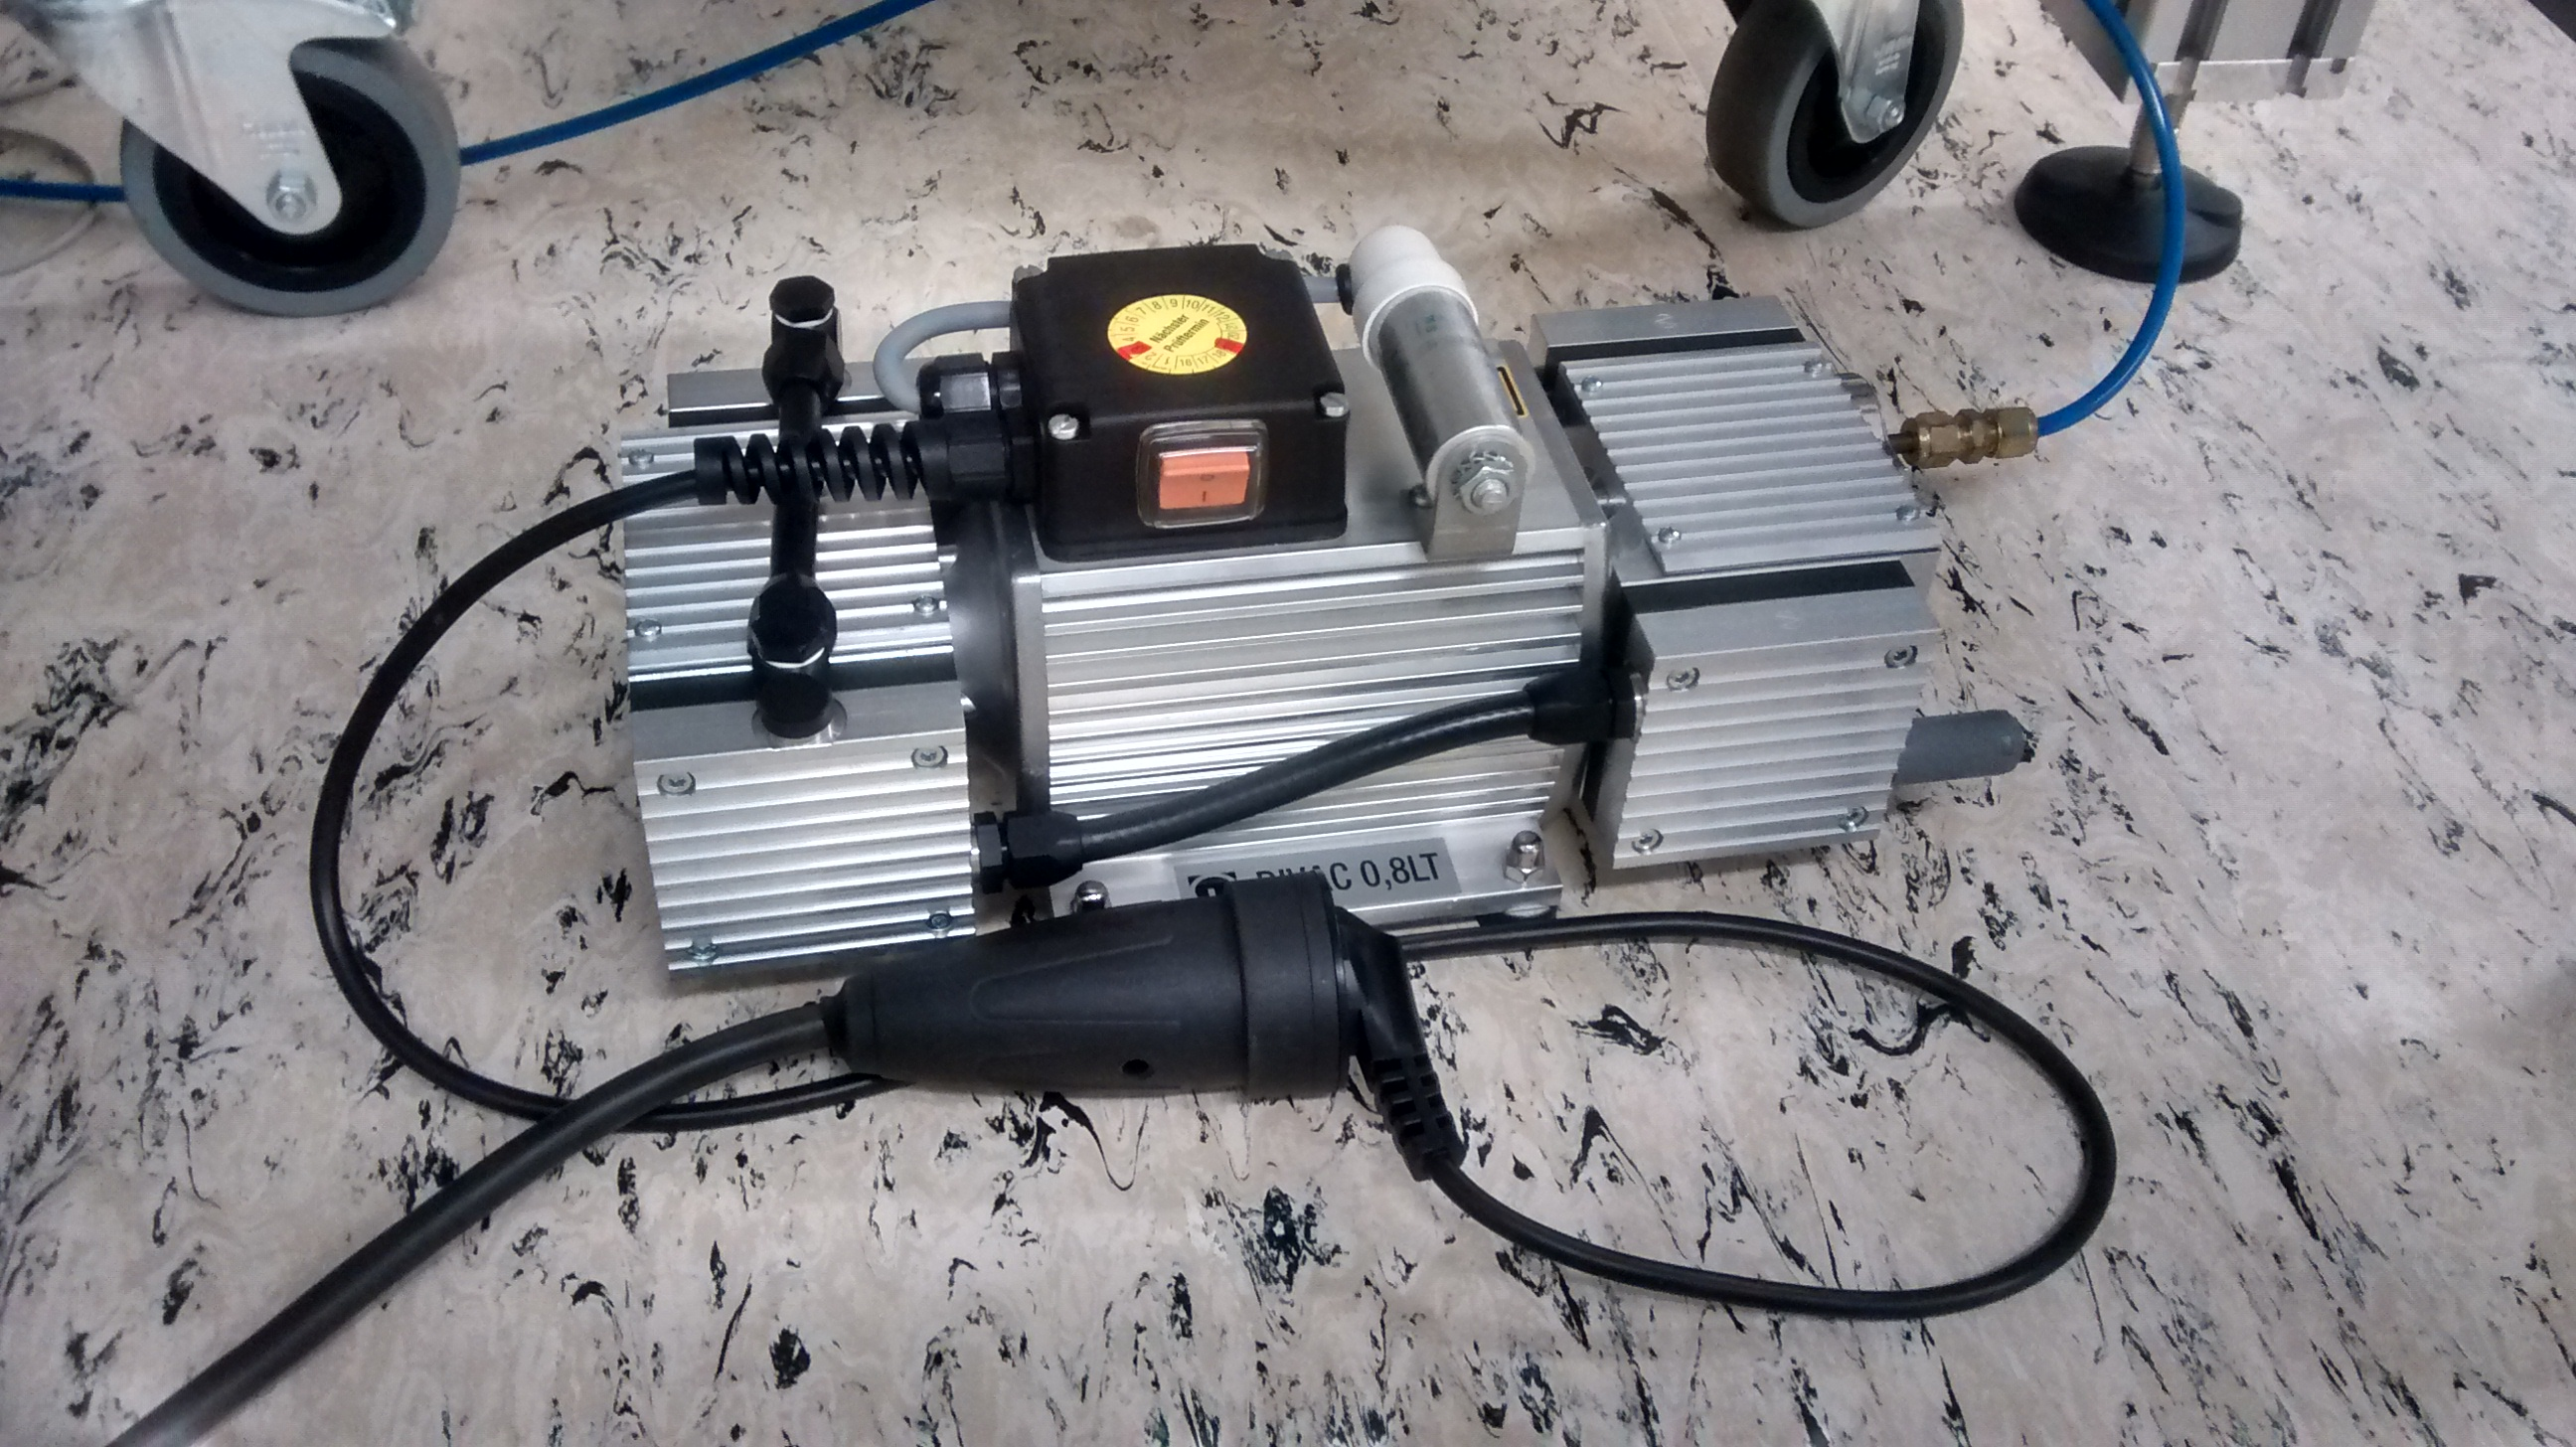
\includegraphics[width=\linewidth]{pictures/compressor.jpg}
\caption[The Compressor]{The compressor on the floor beneath the cold box.}
\label{fig:compressor}
\end{subfigure}
\end{figure}

\subsection{Chuck and XY-Stage}
\label{sec:chuck}

The chuck inside the cold box is connected to the high voltage from the CV/IV box, the vacuum line from the compressor and the coolant inlet and outlet from the chiller.
A dry air connection and a serial cable from the chiller control unit are also connected.
The position of the chuck can be adjusted manually by turning the wheels, the levers allow for larger movements.
When moving the chuck, the probe needles should be well away from the chuck surface as to avoid damage and scratching.\\

\subsection{Probe Needles}
\label{sec:needles}

There are four probe needles on manipulators, sitting on magnetic rails in the cold box.
One needle is for the pad/high voltage connection, one needle for the guard ring connection.
Both these needles are clearly marked.
The two remaining needles are spares or can be used for alternative measurements.
Figure~\ref{fig:needle} shows a manipulator and how to adjust its position.
The probe needles should be handled extremely carefully, as they can break very easily.
They should be far away from any moving objects.
For positioning, the microscope should be used.\\

\begin{figure}[hbtp]
\begin{center}
\begin{overpic}[width=0.70\textwidth,trim=0 0 -5cm -5cm, clip]{pictures/probe.png}
\put(7.5,15){\small Needle}
\put(70,15){\small Magnetic foot}
\put(90,30){\parbox{.5in}{\small Forward/\\backward\\ movement}}
\put(90,40){\parbox{.5in}{\small Left/right\\ movement}}
\put(80,55){\parbox{.5in}{\small Up/down\\ movement}}
\put(55,52){\small Needle force}
\put(30,45){\small Electrical connector}
\end{overpic}
\end{center}
\captionsetup{width=.8\linewidth}%
\captionof{figure}[A Needle Probe]{A needle probe. The bottom screw can be used to adjust the position in forward/backward direction, that is in the direction of the needle. By using the up/down screw, the needle is placed on the device under test.}
\label{fig:needle}
\end{figure}

\subsection{Keithley 6517B}
\label{sec:keithley6517b}

The Keithley 6517B is used as a voltage source for the setup and to measure the DUT currents.
It is controlled by the software running on the read-out computer.
Figures~\ref{fig:keithley6517bfront} and~\ref{fig:keithley6517bback} show the front and back views of the device.
The connection schematic is shown in figure~\ref{fig:electrical} and explained in section~\ref{sec:connections}.
A manual can be downloaded from~\cite{ref:keithley6517bref}.
It can take a while for the Keithley 6517B to warm up after switching it on, so for comparable and accurate measurements it is advised to wait a few minutes.
After a measurement, the Keithley 6517B should be turned off again.\\

\begin{figure}[hbtp]
\centering
\begin{subfigure}[t]{0.475\textwidth}
\centering\captionsetup{width=.8\linewidth}%
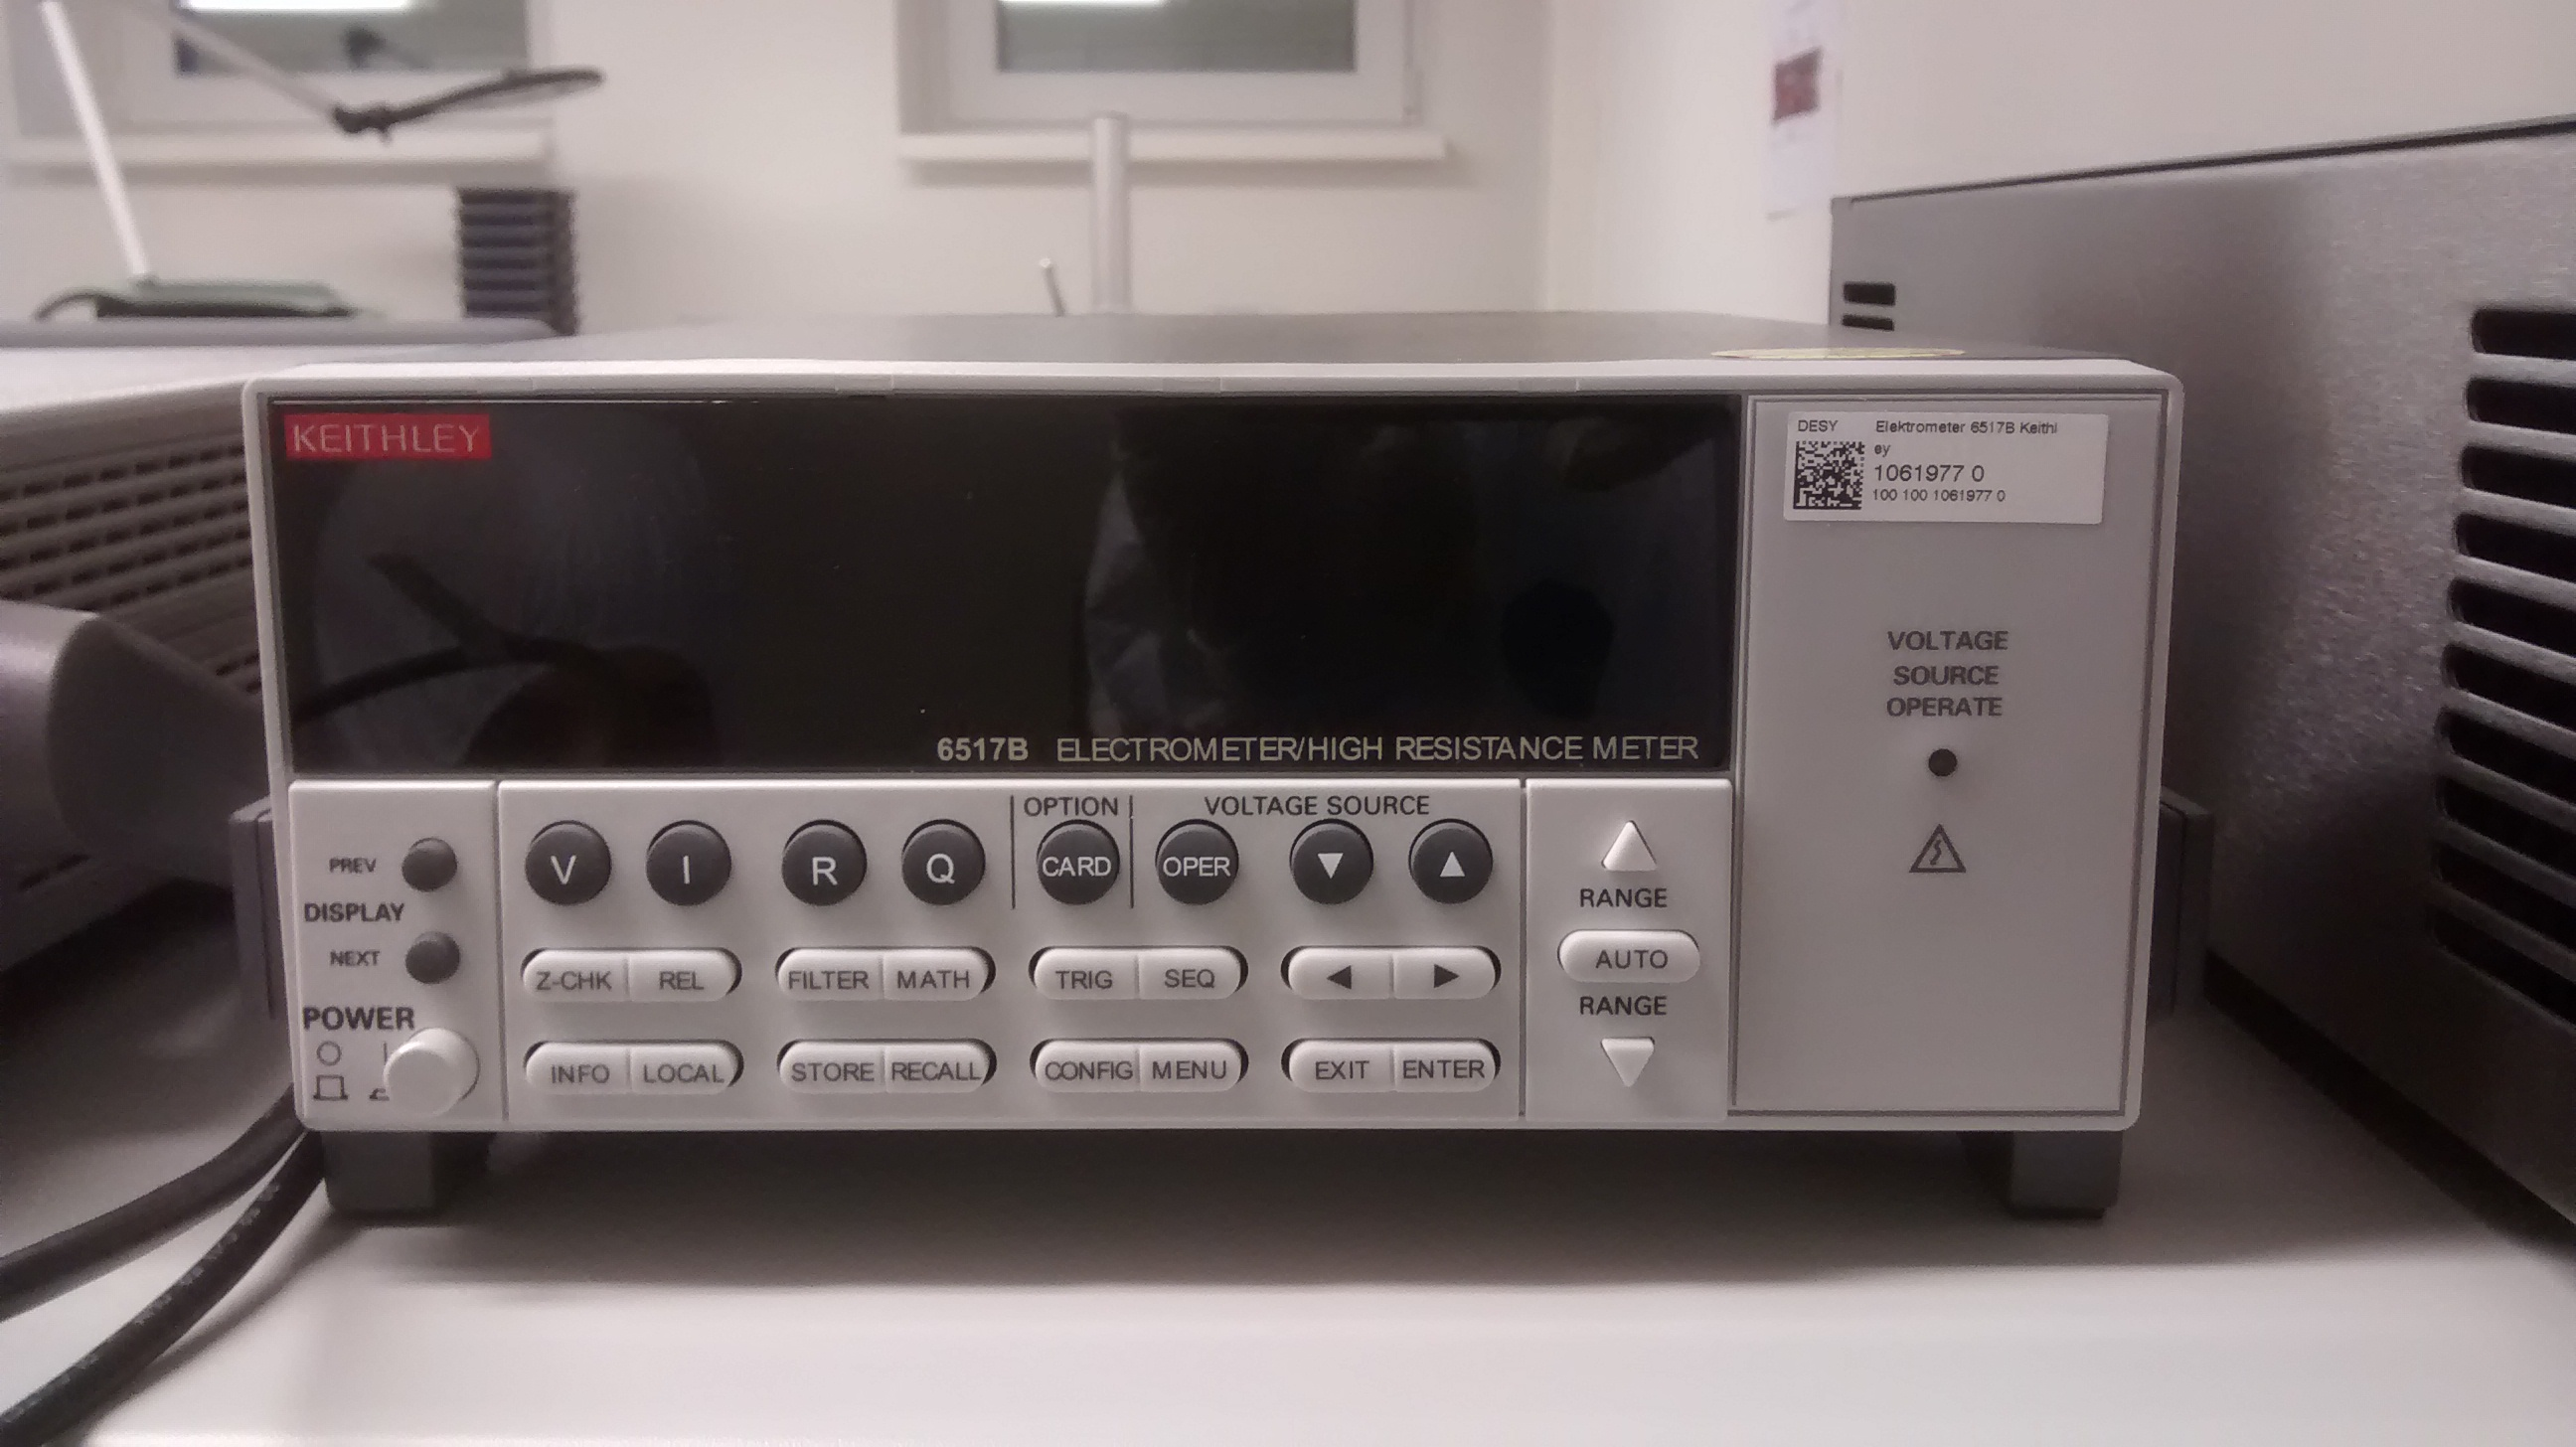
\includegraphics[width=\linewidth]{pictures/front_keithley65.jpg}
\caption[Front View of the Keithley 6517B]{Front view of the Keithley 6517B. The on/off switch is at the bottom left.}
\label{fig:keithley6517bfront}
\end{subfigure}
\begin{subfigure}[t]{0.475\textwidth}
\centering\captionsetup{width=.8\linewidth}%
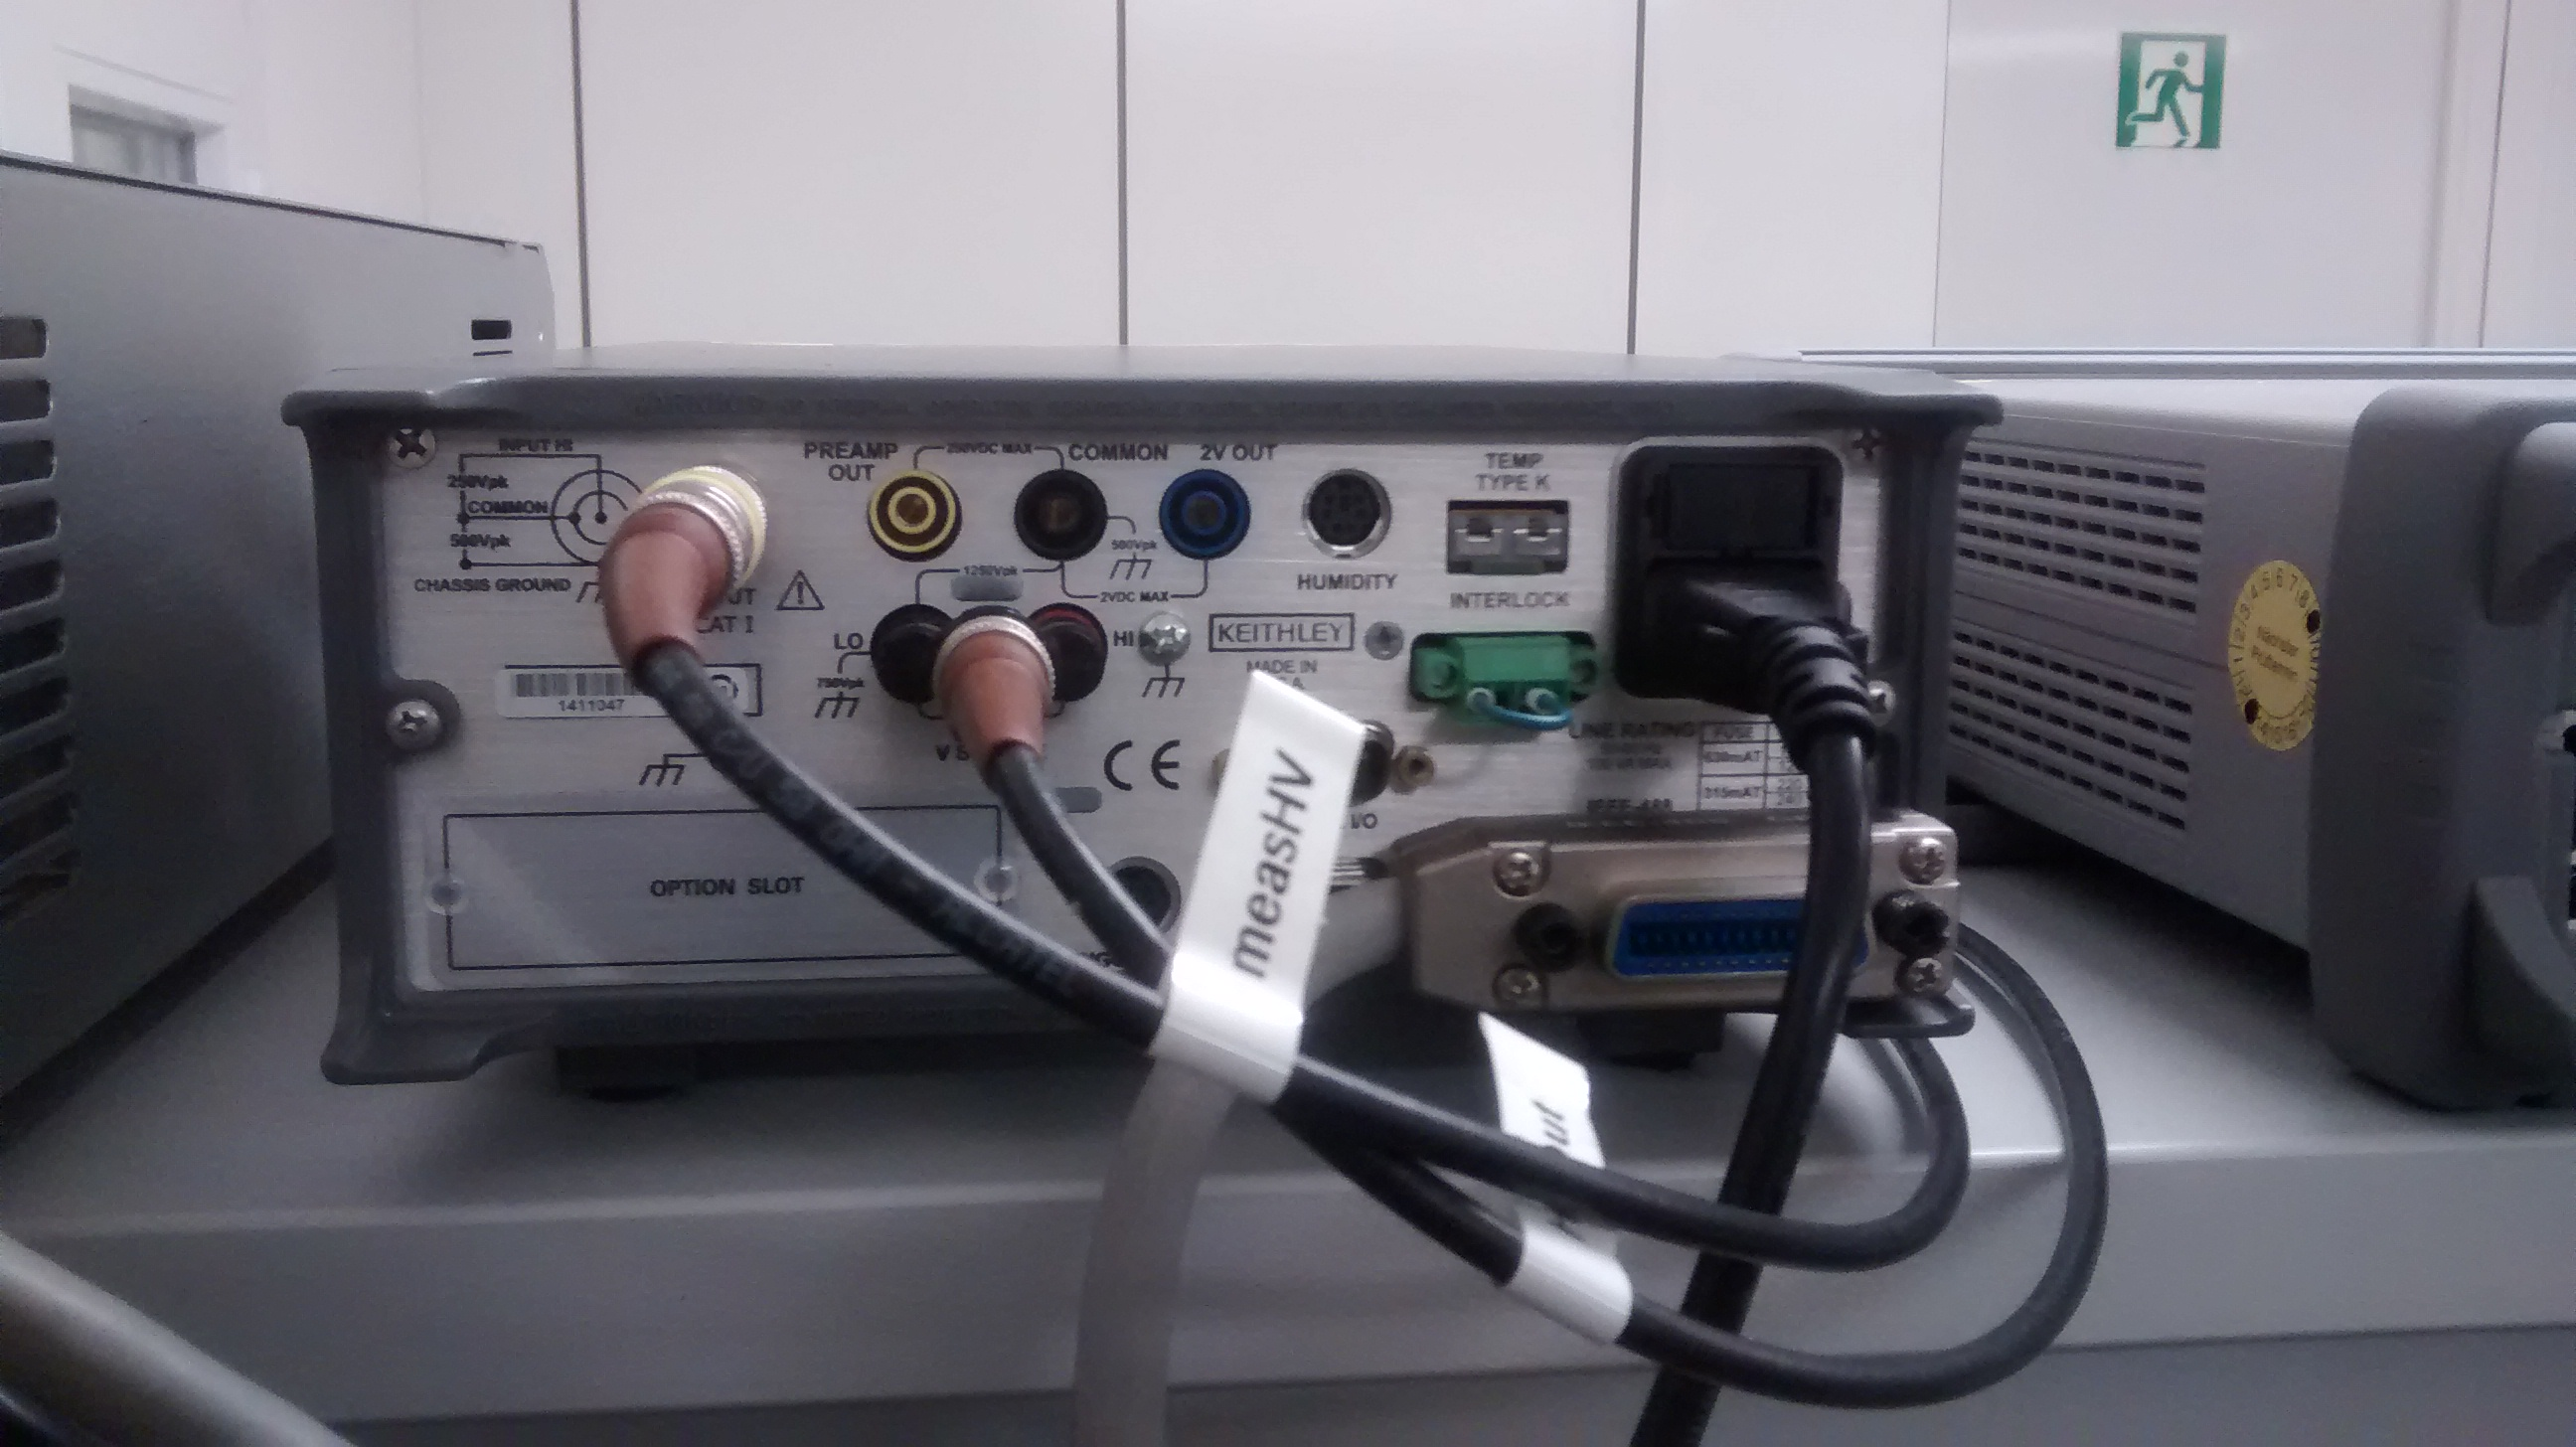
\includegraphics[width=\linewidth]{pictures/back_keithley65.jpg}
\caption[Back View of the Keithley 6517B]{Rear view of the Keithley 6517B. The cable labelled {\tt ImeasHV} goes to the top left triax input connector. The source outputs connect to the {\tt HVout} cable.}
\label{fig:keithley6517bback}
\end{subfigure}
\end{figure}

\subsection{Agilent E4980A and the CV/IV Box}
\label{sec:agilent}

The Agilent E4980A LCR-Meter is used for capacitance measurements.
Via the CV/IV box it can be switched into the connection between the Keithley 6517B and the DUT/chuck.
A manual can be downloaded from~\cite{ref:agilentref}.
The CV/IV box shown in figure~\ref{fig:cvivbox} is plugged into the front of the Agilent E4980A and allows the user to select between IV (bottom switch to top) and CV (bottom switch to bottom) measurement modes.
The top switch can be used to connect (${\rm C_{int}}$) or disconnect (${\rm R_{int}}$) the Agilent E4980A to the top row connectors.
Switching should {\bf never} be done during a measurement or whilst a voltage is applied.
Note that if the CV/IV box is in CV mode, the current measurement of the Keithley 6517B will no longer be accurate.
This is because of the large internal resistance of the Agilent E4980A and the CV/IV box.
Thus, the following operation modes are available:\\

\begin{itemize}
\item{{\bf IV Mode:\\}}
The bottom switch is in the top position ({\tt IV}).
The position of the top switch is not relevant as only the Keithley 6517B and optionally the Keithley 6485 are used.

\item{{\bf CV Mode:\\}}
The bottom switch is in the bottom position ({\tt CV}), the top switch is in the top position (${\tt R_{int}}$).
The Keithley 6517B and the Agilent E4980A are used via a single probe needle.

\item{${\rm {\bf C_{int}}}$ {\bf Mode:\\}}
The bottom switch is in the top position ({\tt IV}), the top switch is in the bottom position (${\tt C_{int}}$).
The Keithley 6517B and the Agilent E4980A are used via different probe needles.

\item{${\rm {\bf R_{int}}}$ {\bf Mode:\\}}
The bottom switch is in the top position ({\tt IV}), the top switch is in the top position (${\tt R_{int}}$).
The Keithley 6517B and an optional external device are usable.
\end{itemize}


\begin{figure}[hbtp]
\centering
\begin{subfigure}[t]{0.475\textwidth}
\centering\captionsetup{width=.8\linewidth}%
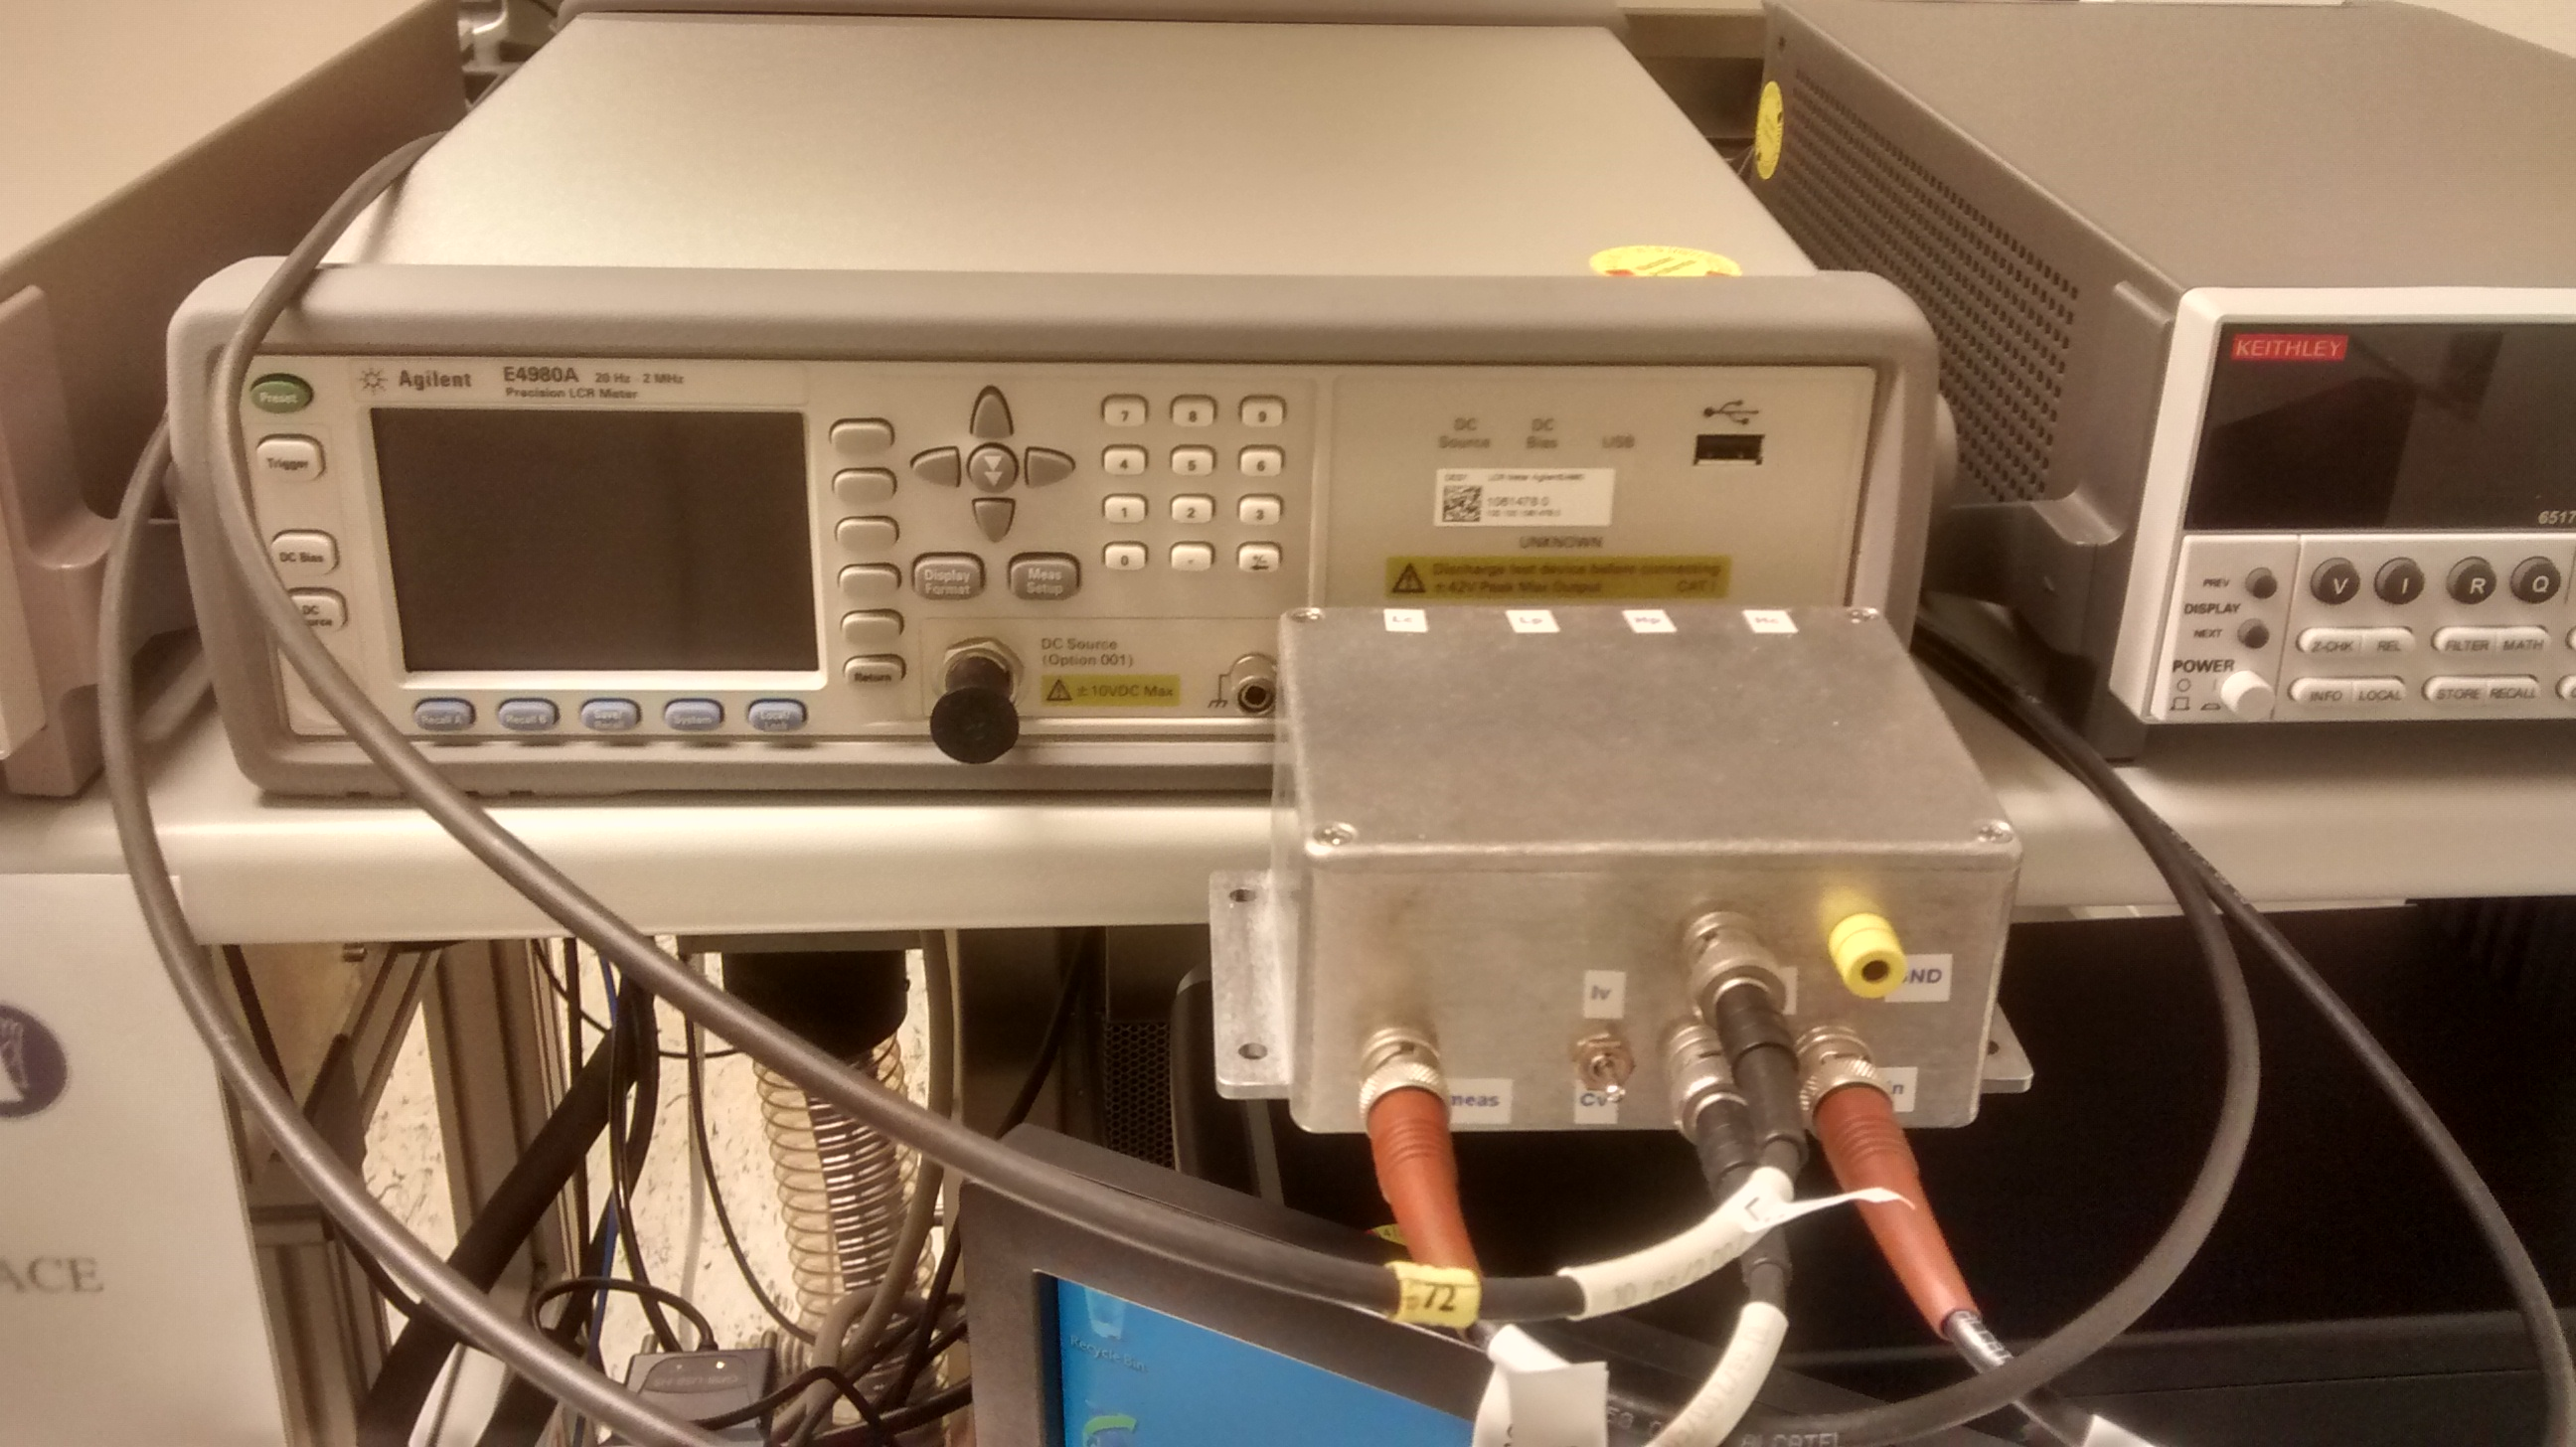
\includegraphics[width=\linewidth]{pictures/front_agilent.jpg}
\caption[Front View of the Agilent E4980A]{Front view of the Agilent E4980A with the old CV/IV box attached. The on/off switch is at the bottom left of the device.}
\label{fig:agilent}
\end{subfigure}
\begin{subfigure}[t]{0.475\textwidth}
\centering\captionsetup{width=.8\linewidth}%
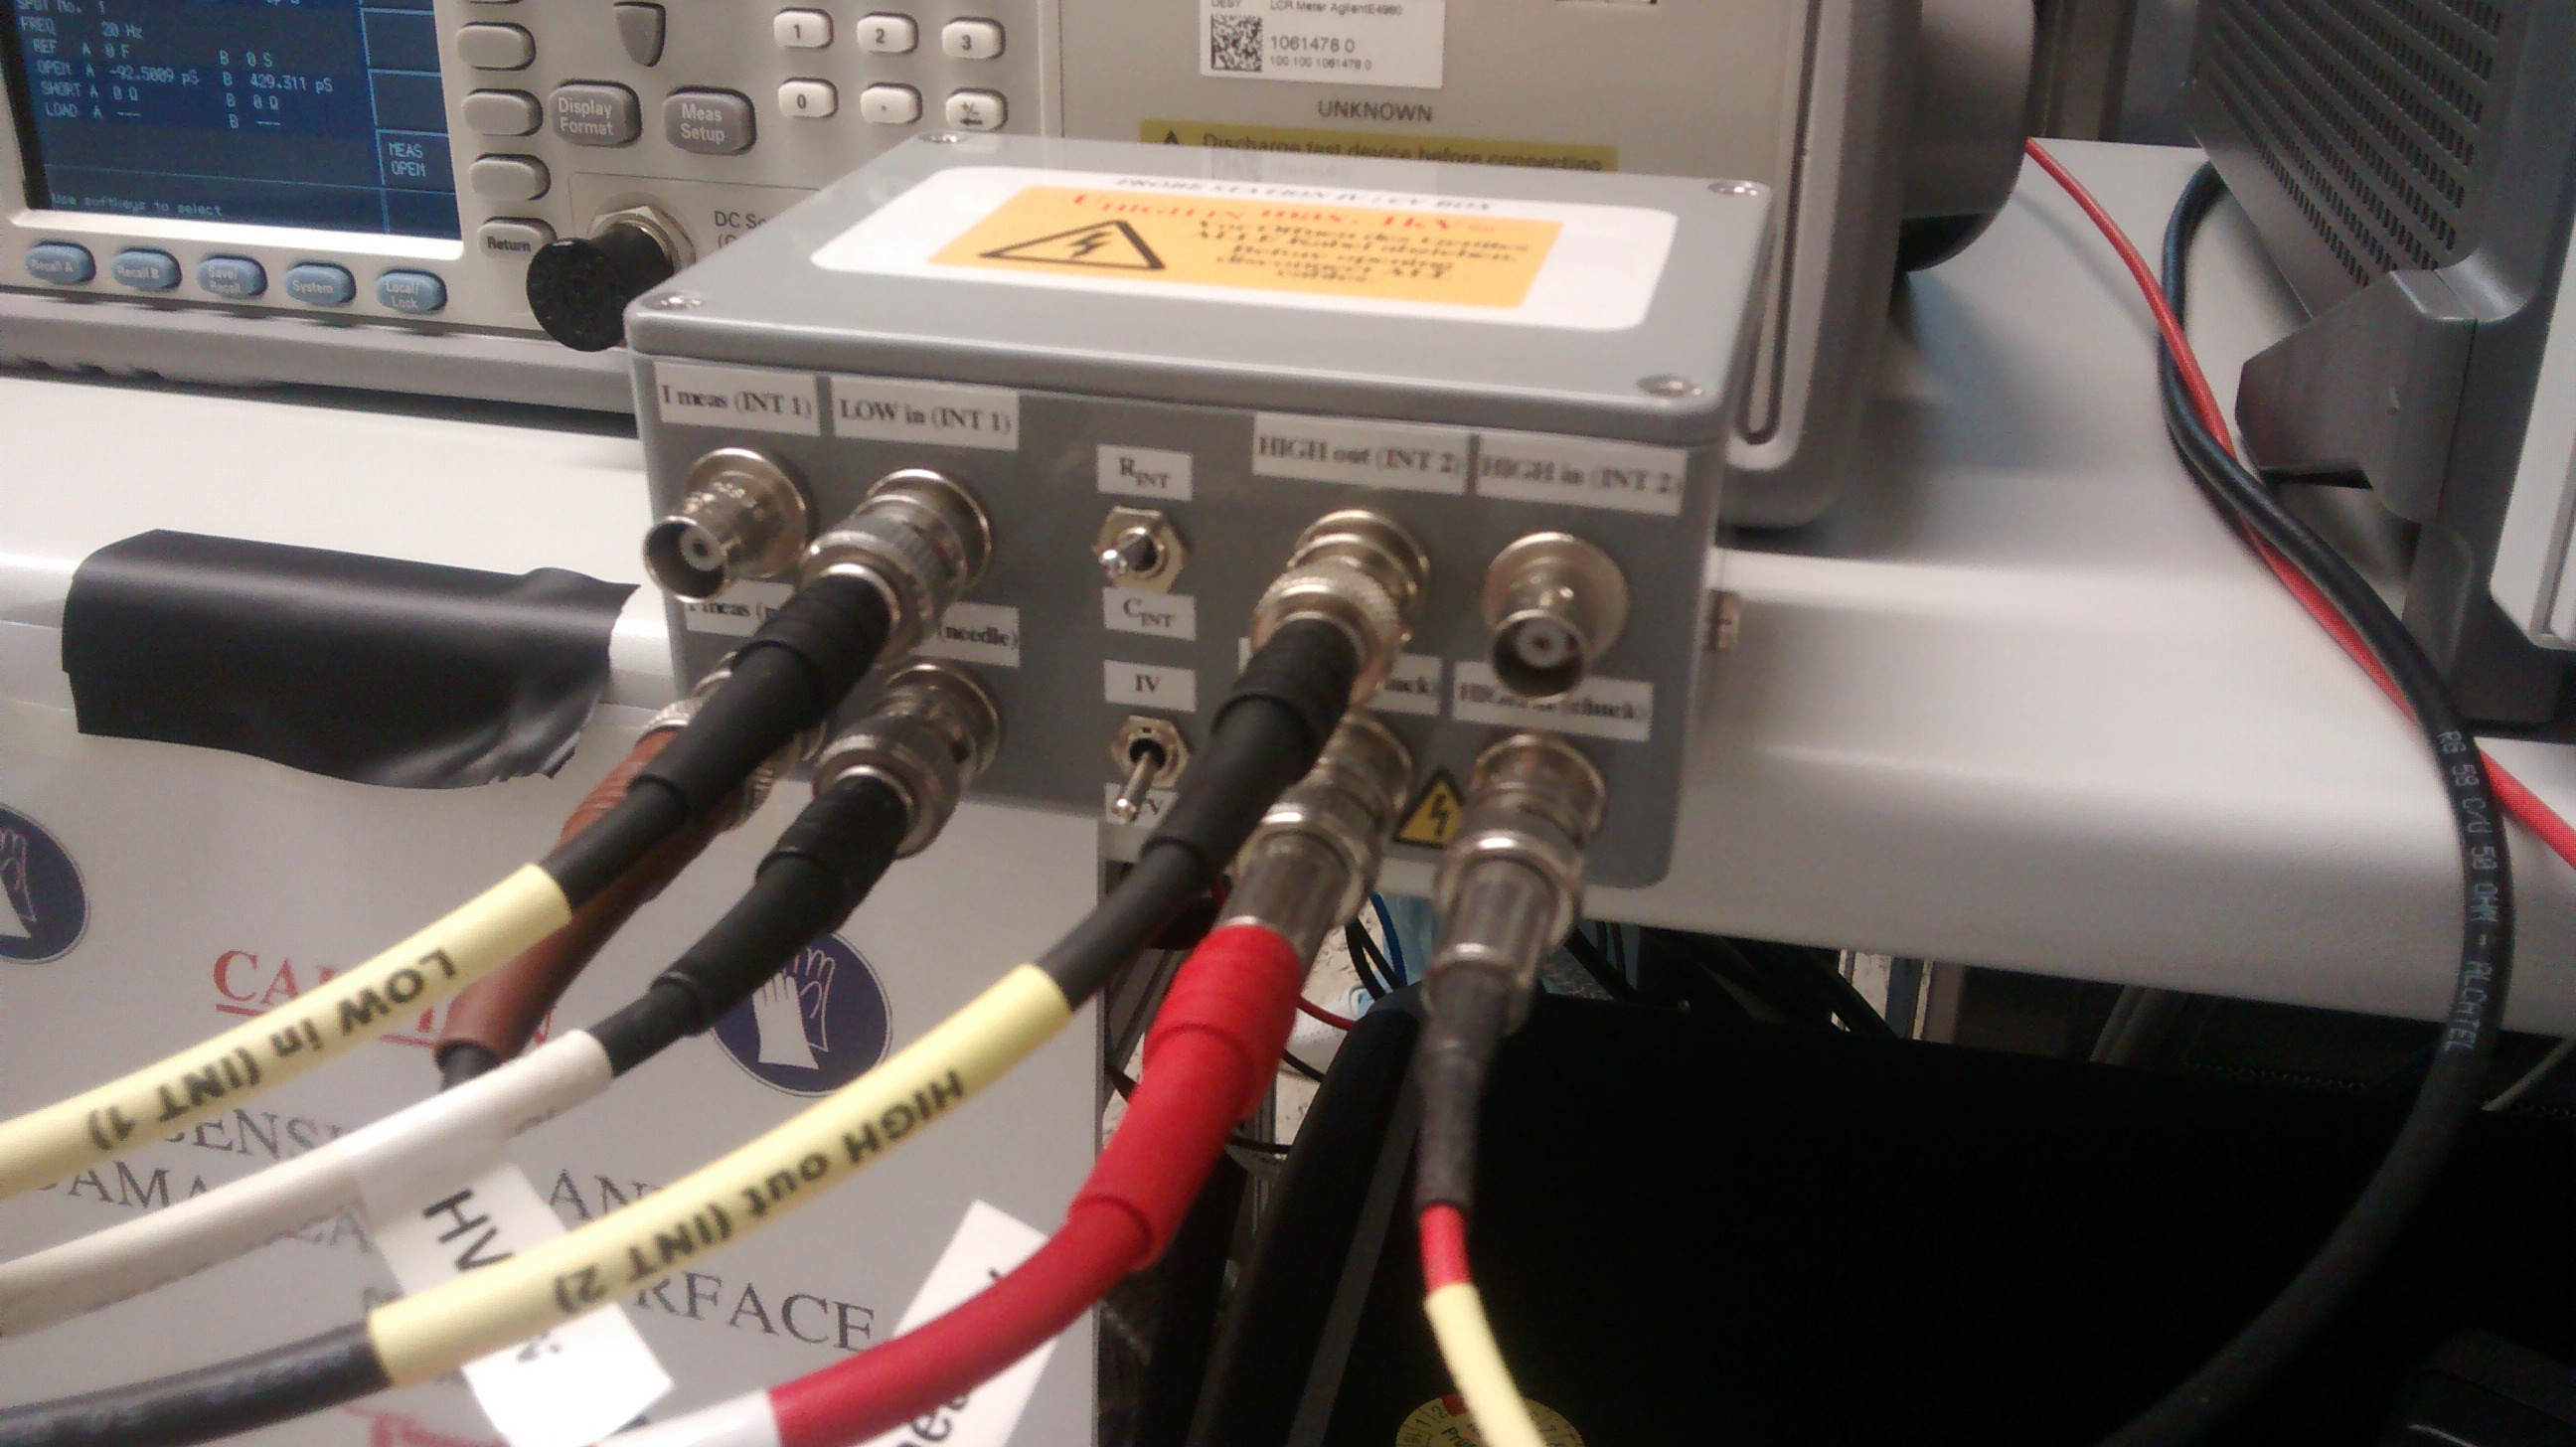
\includegraphics[width=\linewidth]{pictures/cvivswitch2.jpg}
\caption[The CV/IV Box]{Close-up of the CV/IV Box. A description of all the connections can be found in section~\ref{sec:connections}.}
\label{fig:cvivbox}
\end{subfigure}
\end{figure}

\subsection{Keithley 6485}
\label{sec:keithley6485}

The Keithley 6485 Picoammeter shown in figures~\ref{fig:keithley6485front} and~\ref{fig:keithley6485rear} is used to measure guard ring currents.
Its usage is optional for IV measurements and it is not needed for CV measurements.
A manual can be found at~\cite{ref:keithley6485ref}.
The Keithley 6485 can also take a while to warm up after powering on, so also here for comparable and accurate measurements it is advised to wait a few minutes.\\

\begin{figure}[hbtp]
\centering
\begin{subfigure}[t]{0.475\textwidth}
\centering\captionsetup{width=.8\linewidth}%
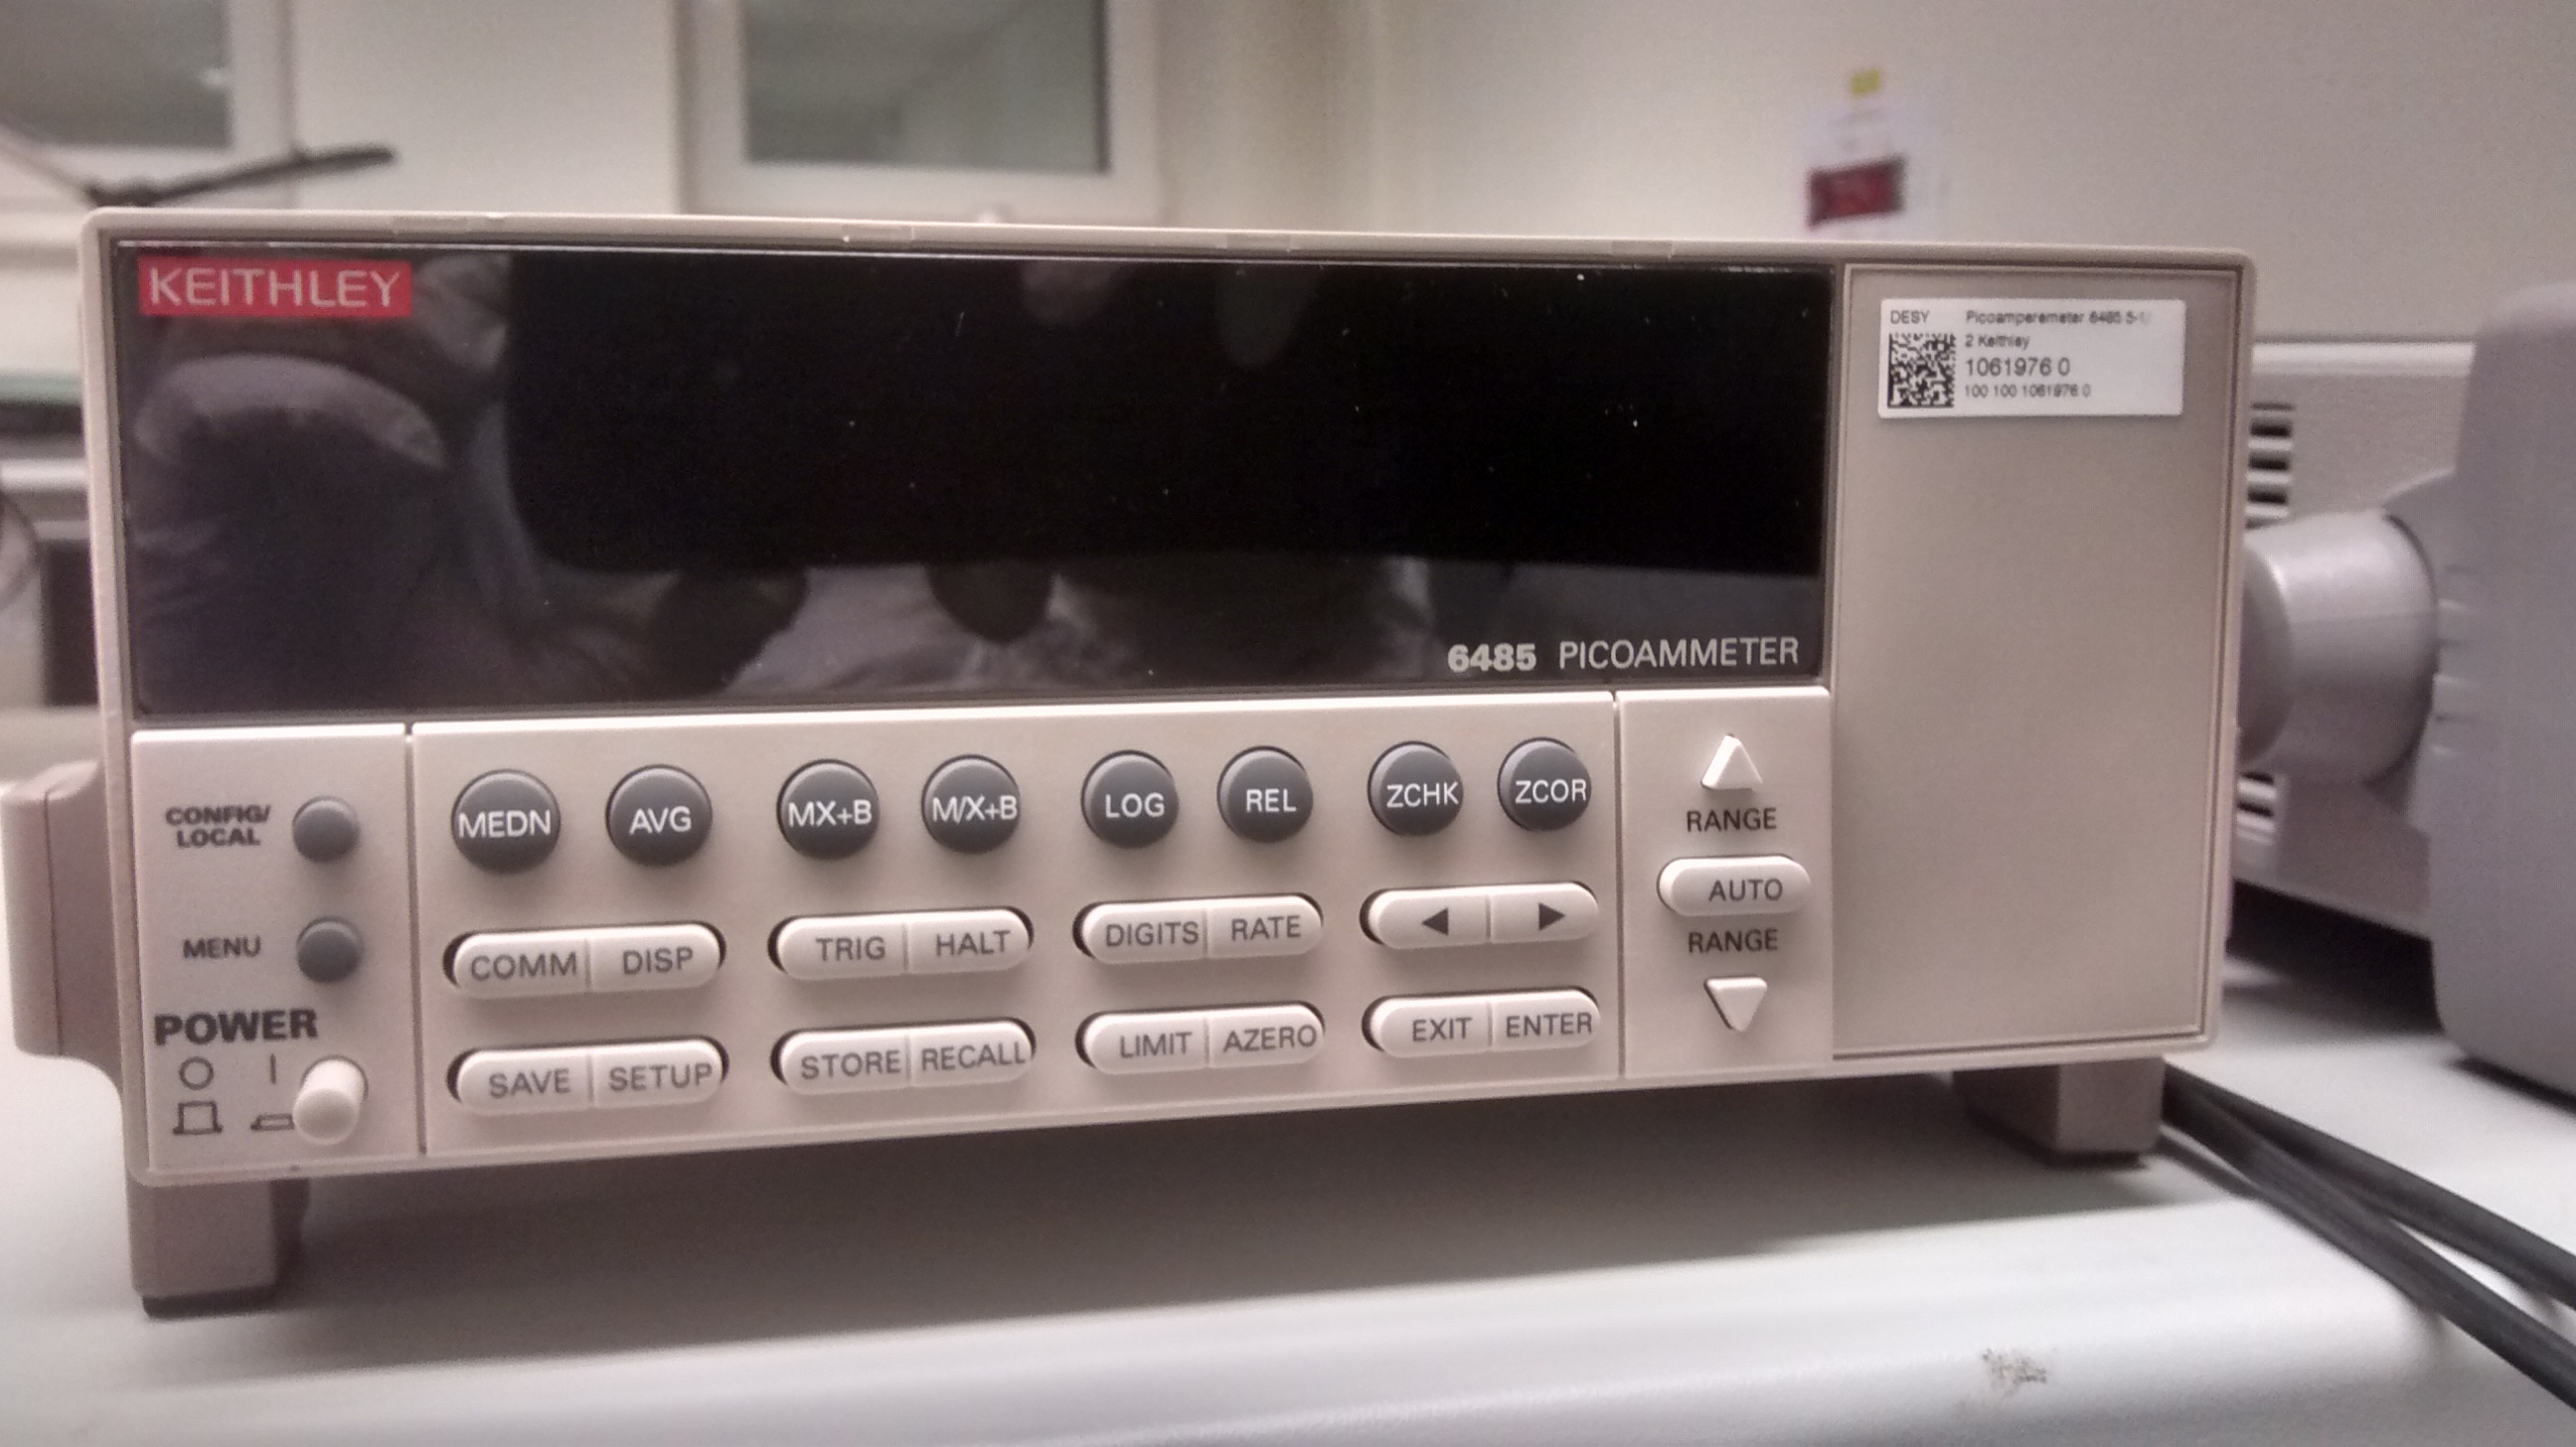
\includegraphics[width=\linewidth]{pictures/front_keithley64.jpg}
\caption[Front View of the Keithley 6485]{Front view of the Keithley 6485. The on/off switch is at the bottom left.}
\label{fig:keithley6485front}
\end{subfigure}
\begin{subfigure}[t]{0.475\textwidth}
\centering\captionsetup{width=.8\linewidth}%
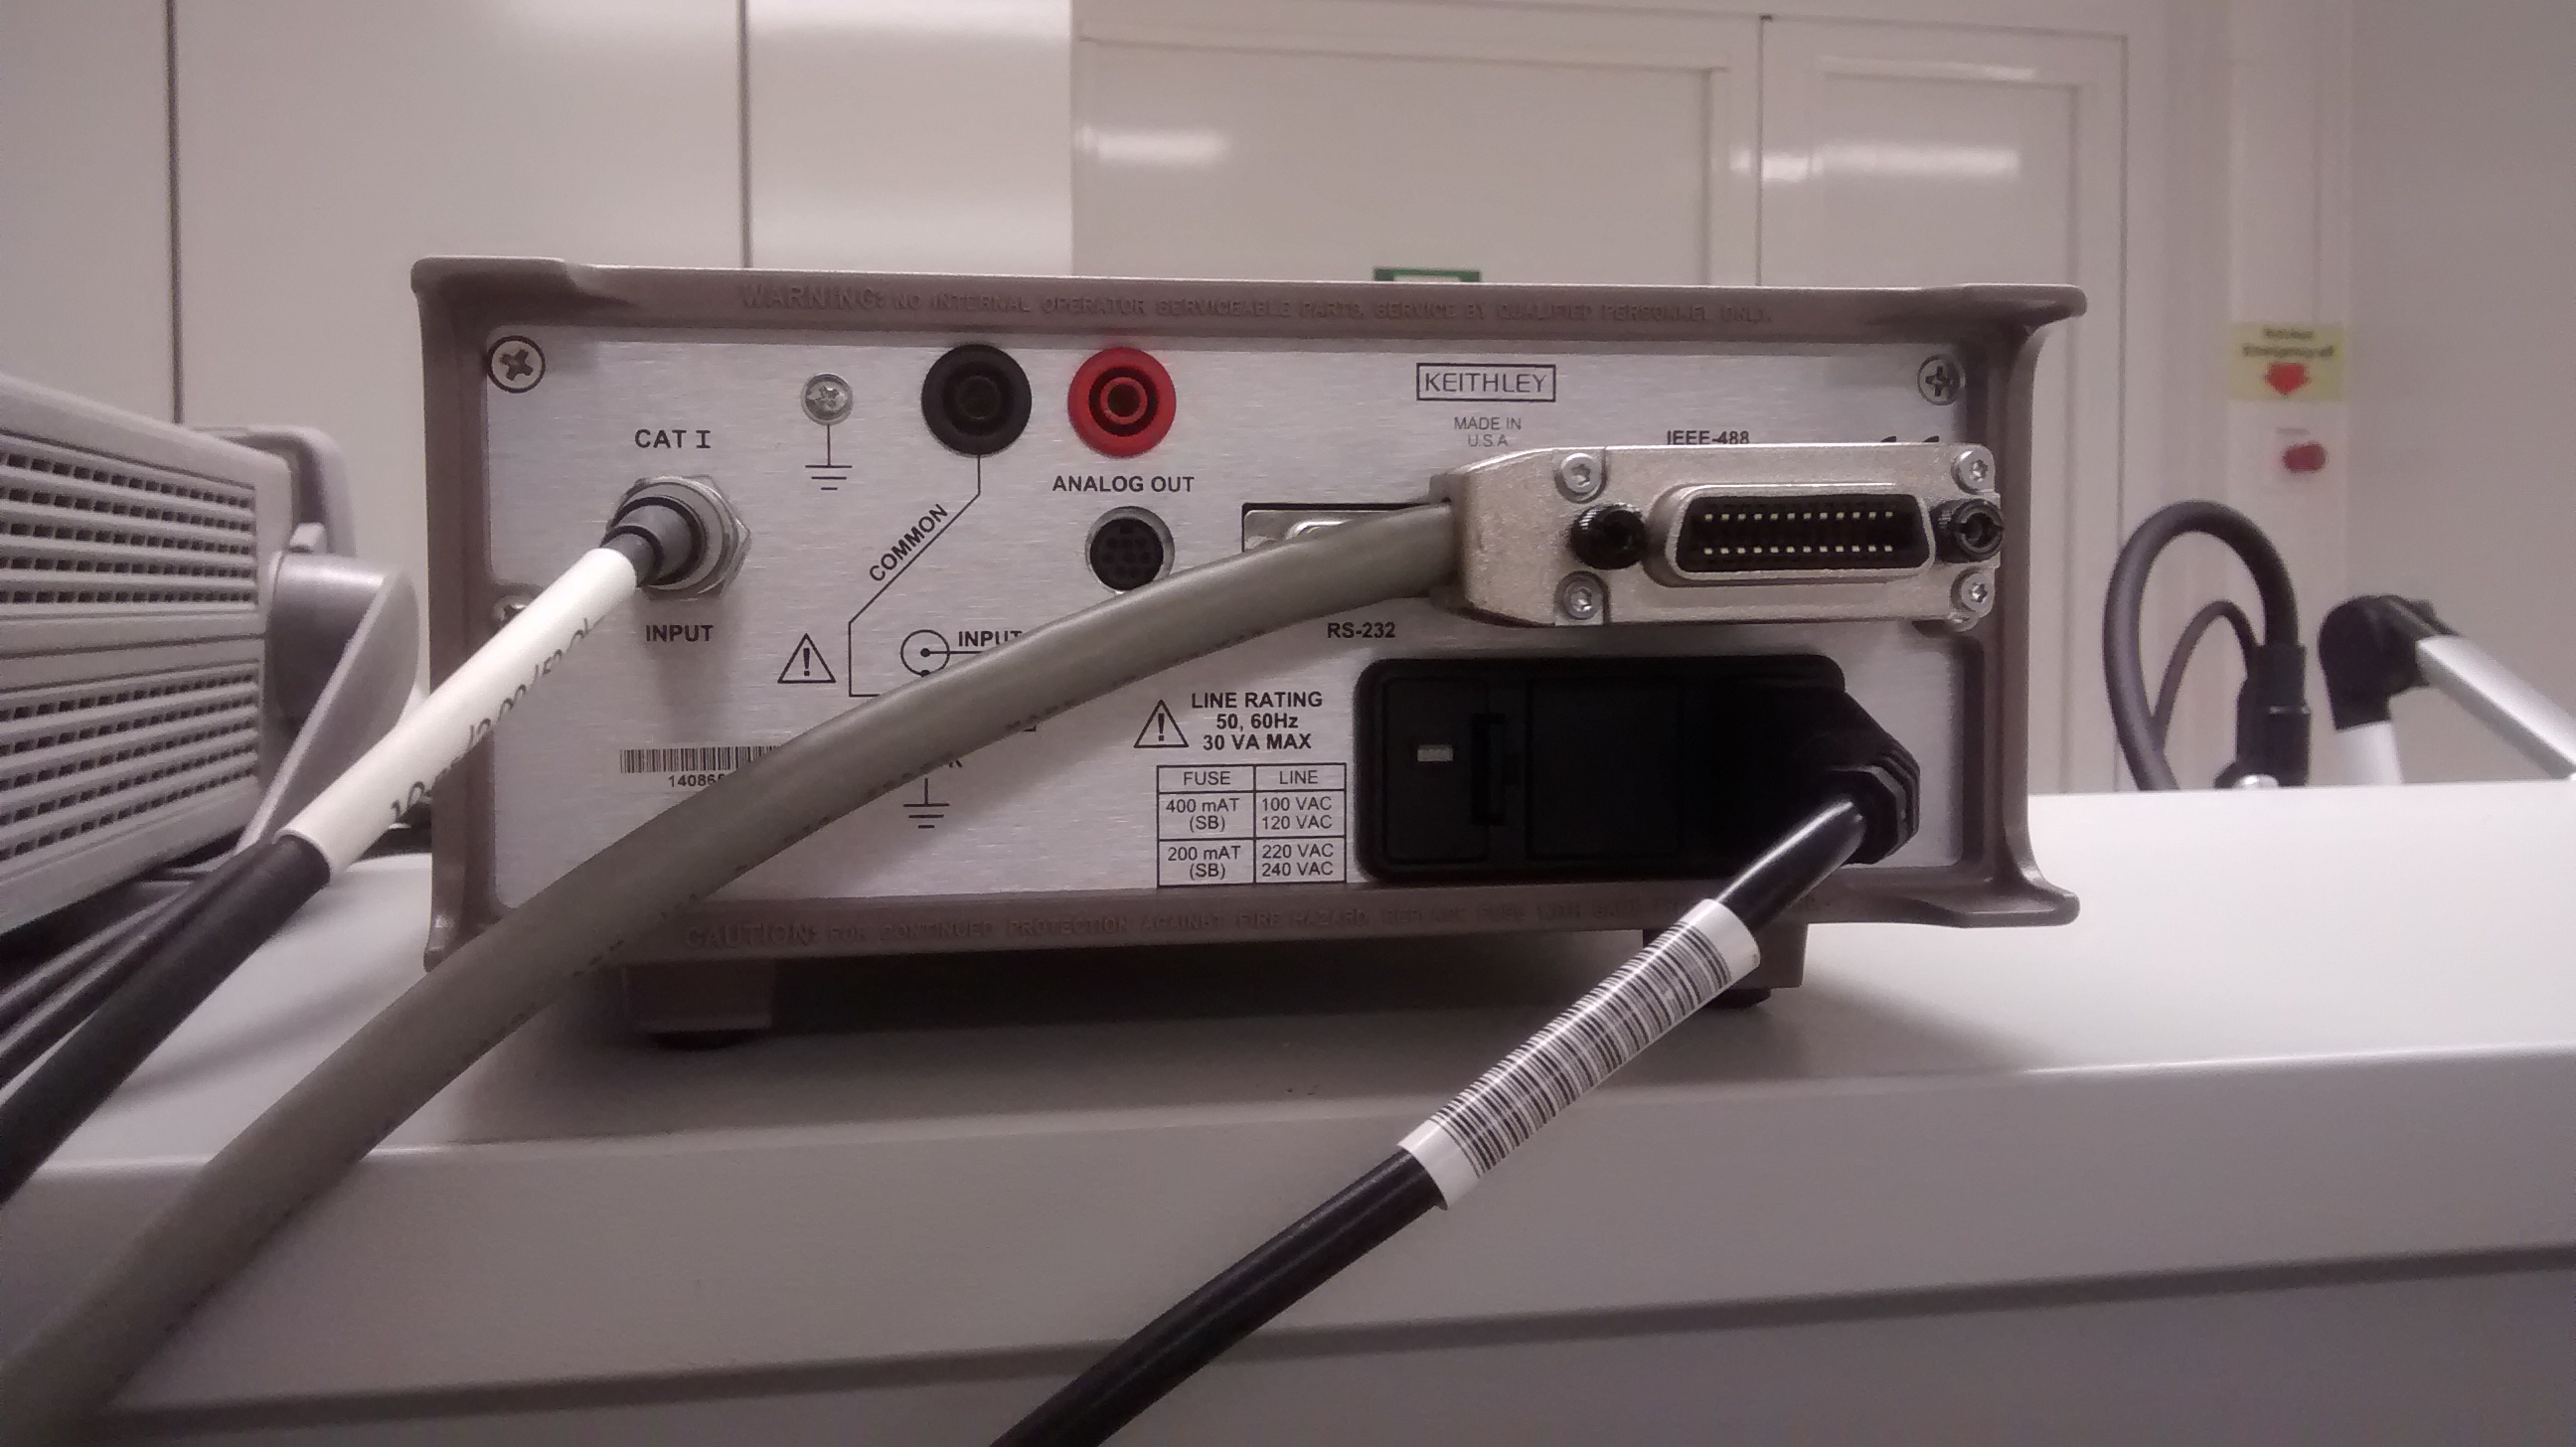
\includegraphics[width=\linewidth]{pictures/back_keithley64.jpg}
\caption[Back View of the Keithley 6485]{Rear view of the Keithley 6485. The cable labelled {\tt Iguard} goes to the input connector.}
\label{fig:keithley6485rear}
\end{subfigure}
\end{figure}

\subsection{Chiller and Control Unit}
\label{sec:chiller}

The chiller can be used to cool the chuck and thus the DUT.
It is switched on by the large red switch on its front.
The chiller control unit (c.f. figures~\ref{fig:attfront} and~\ref{fig:attback} for front and back views) is located on the shelf above the read-out computer and has a power switch on its rear.
The control unit is operated via the front touch pad.
Beware that to operate the chiller, it must have sufficient coolant inside.
Furthermore, to prevent condensation, the cold box should be flushed with dry air.
To monitor the dew point, a pipe with dry air is routed into the chiller control unit and from there into the chuck.
Inside the cold box, a dew point sensor probe connected to the control unit (connector {\tt X5}) measures temperature and humidity.
Two serial cables (attached at connectors {\tt X4} and {\tt X7}) connect the chiller control unit to the chiller (connectors there {\tt X8} and {\tt X9}).
The large DIN connector ({\tt X2}) is connected to the chuck and can be used for heating the chuck and for temperature read-out.
Whilst there is a GPIB connection to the read-out computer, a computer-controlled operation has not yet been implemented.
An overview of the dry air and chiller connections is shown in figure~\ref{fig:dryair} in section~\ref{sec:connections}.\\

\begin{figure}[hbtp]
\centering
\begin{subfigure}[t]{0.475\textwidth}
\centering\captionsetup{width=.8\linewidth}%
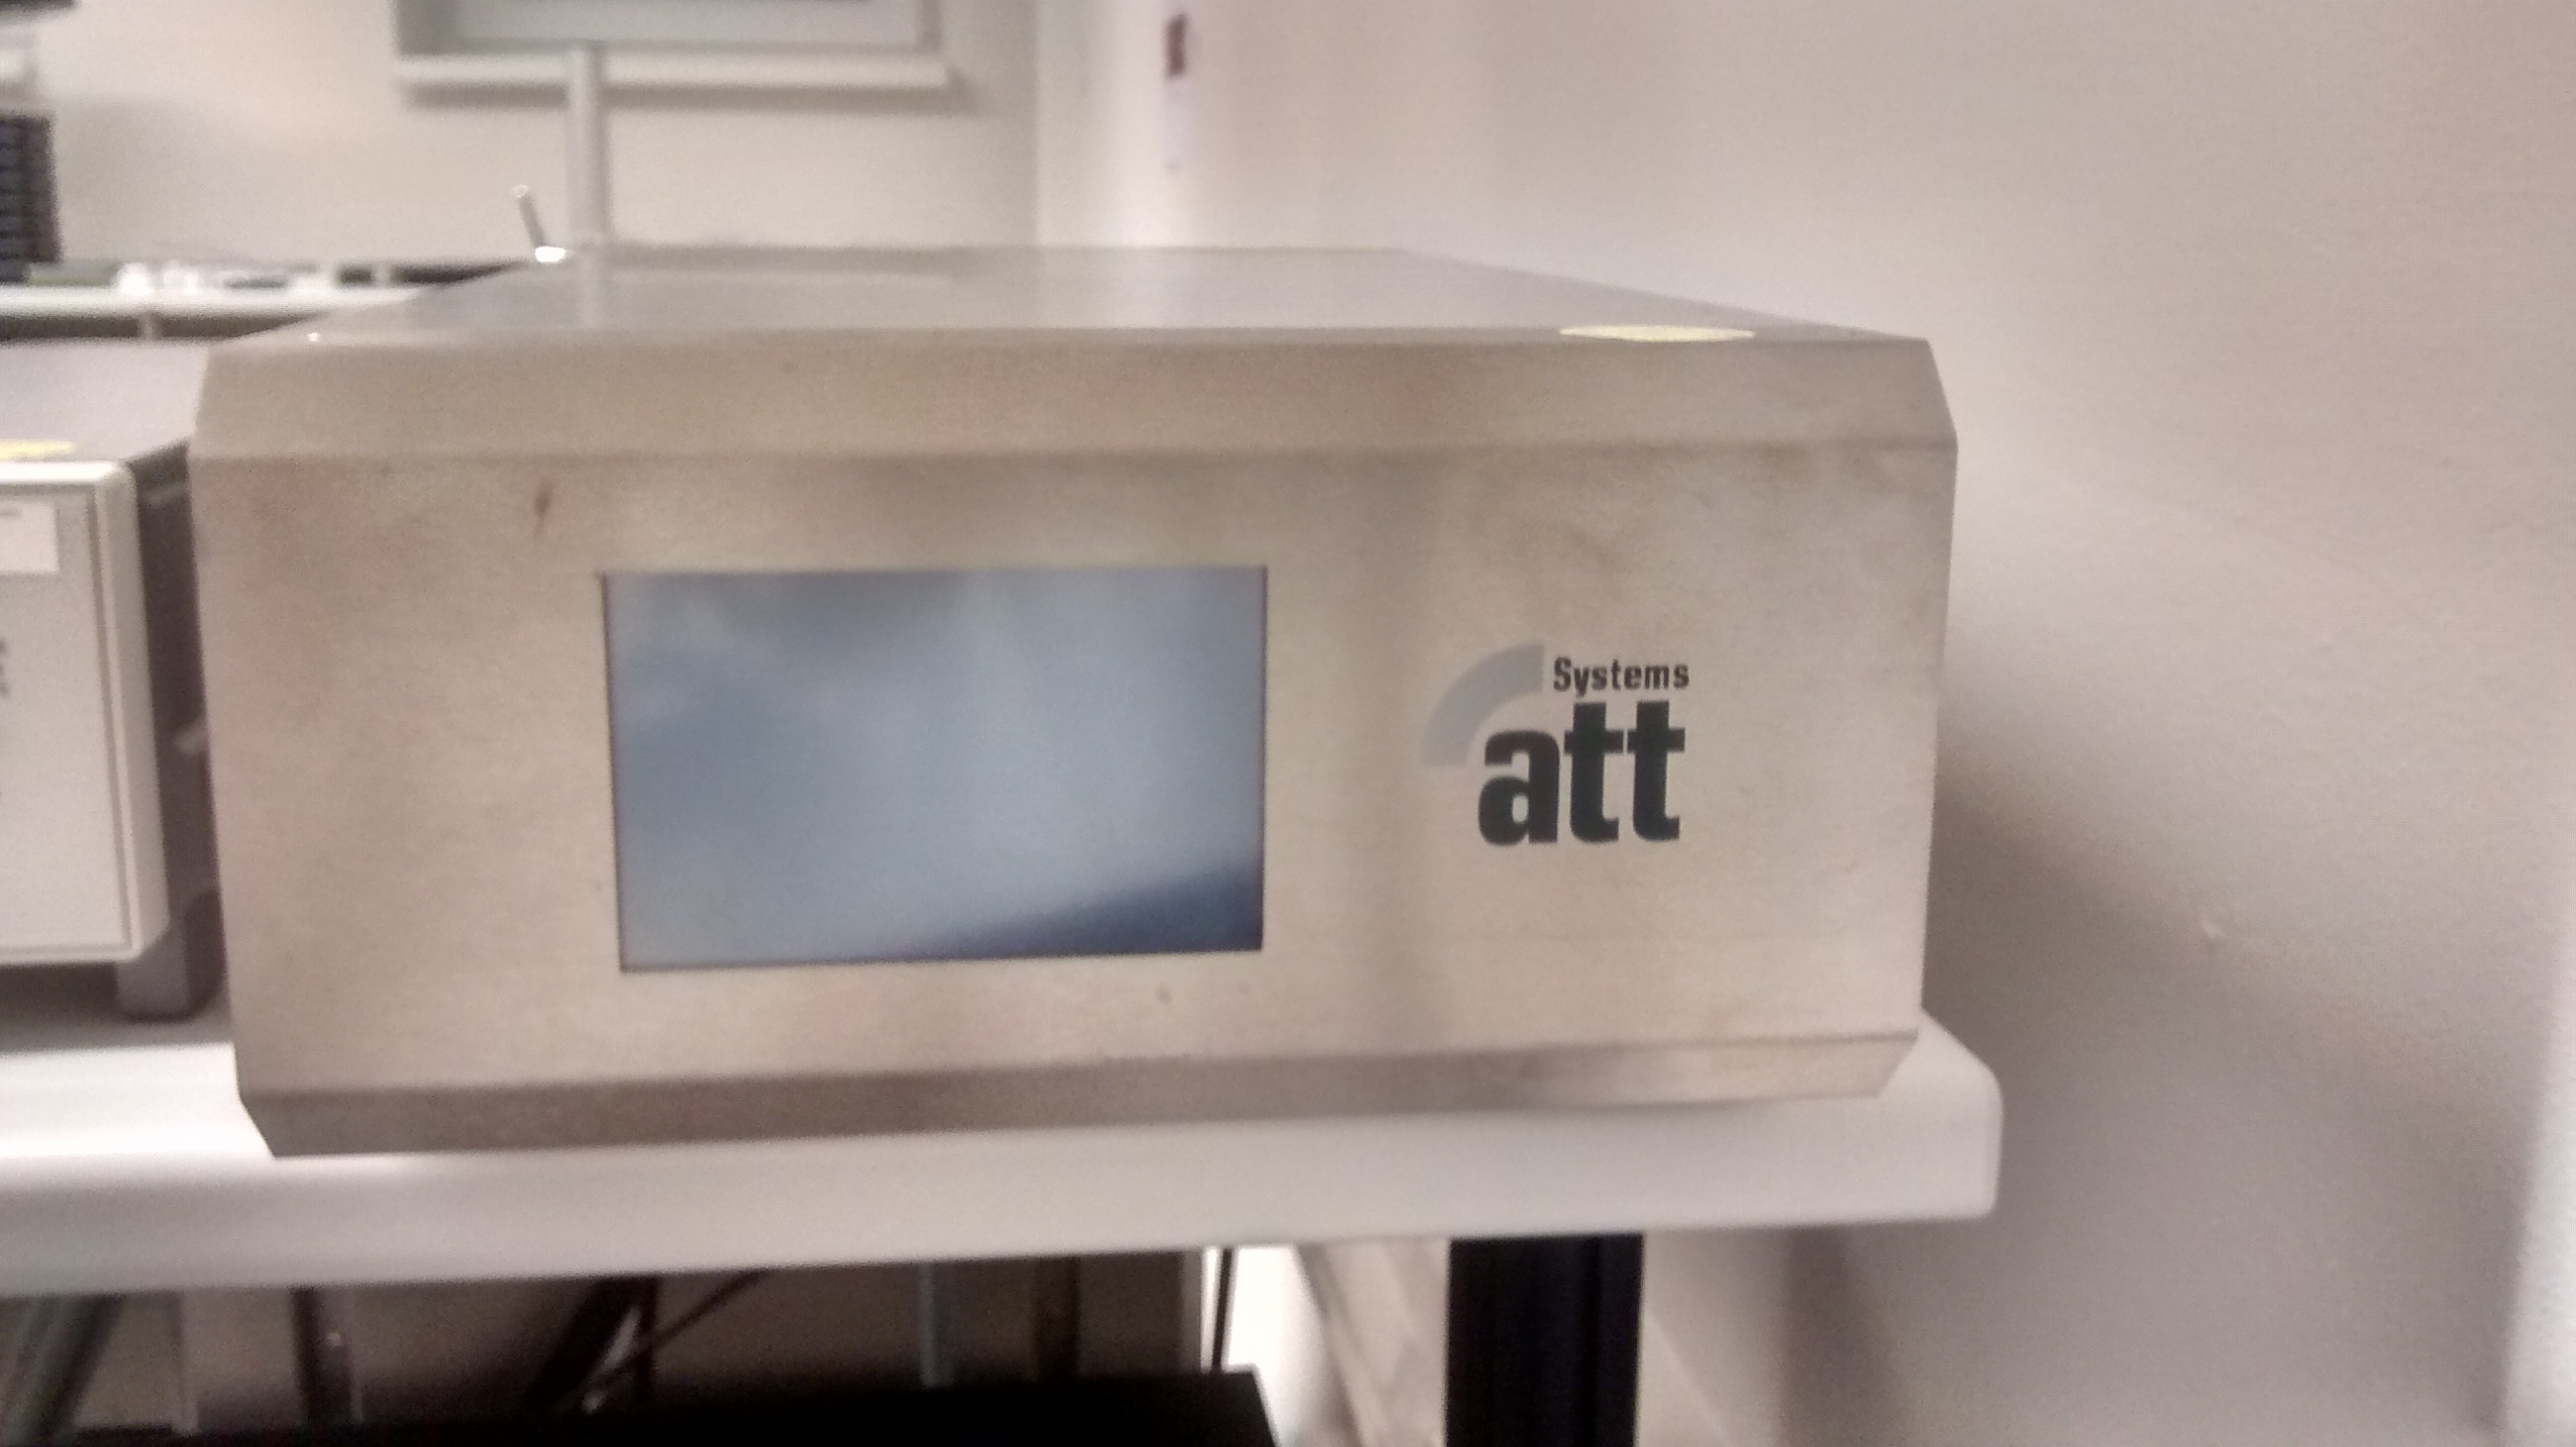
\includegraphics[width=\linewidth]{pictures/att_front.jpg}
\caption[Front View of the Chiller Control Unit]{Front view of the chiller control unit. It is operated via the touch-pad screen.}
\label{fig:attfront}
\end{subfigure}
\begin{subfigure}[t]{0.475\textwidth}
\centering\captionsetup{width=.8\linewidth}%
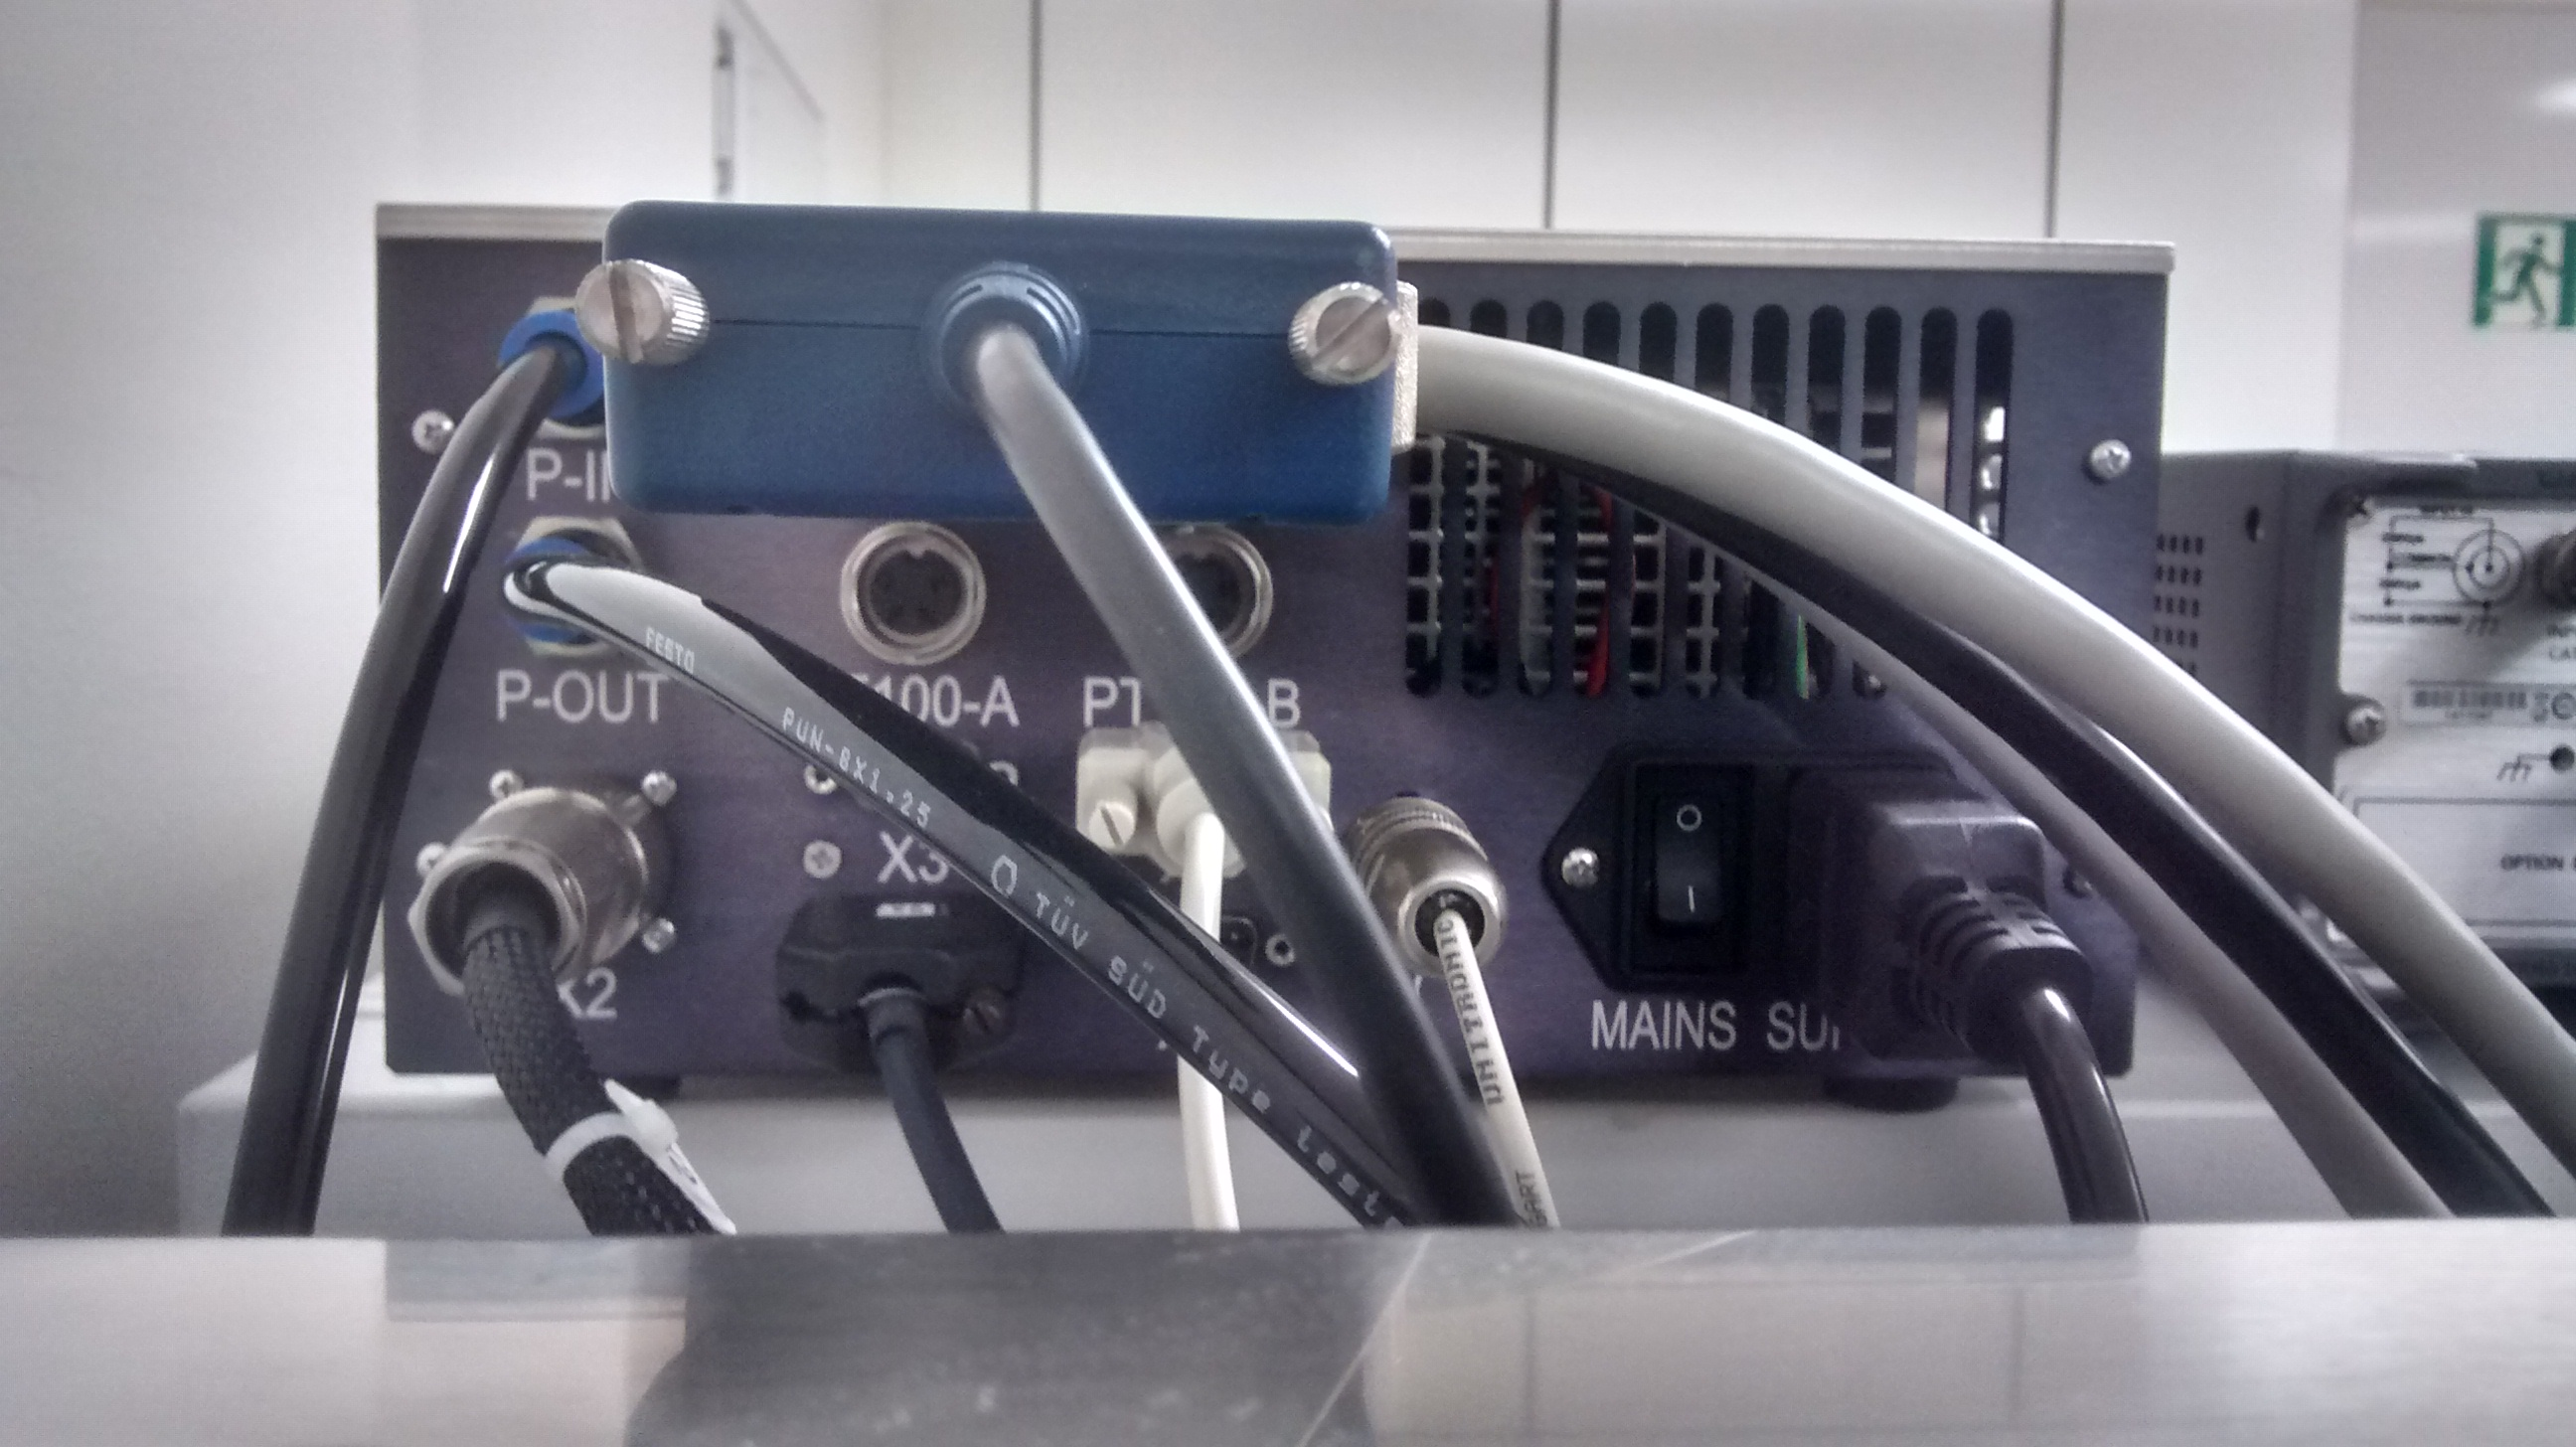
\includegraphics[width=\linewidth]{pictures/att_back.jpg}
\caption[Back View of the Chiller Control Unit]{Rear view of the chiller control unit. The on/off switch is located at the bottom right.}
\label{fig:attback}
\end{subfigure}
\end{figure}

\subsection{Read-Out Computer}
\label{sec:computer}

The read-out computer (computer name: {\tt fhlprobest.desy.de}) is connected to the measurement devices via an GPIB-to-USB connector.
As the operating system is Windows 7, a login is only possible if your DESY user account is in the group {\tt win}.
Your group administrator or the UCO can add you to this group.
Also, a remote connection is possible via the {\tt rdp} protocol if your account is in the group {\tt winterm}, so you can remotely connect to the read-out computer via the command

\medskip
\begin{lstlisting}
xfreerdp --ignore-certificate -u my-user-name -d win fhlprobest.desy.de
\end{lstlisting}
\medskip

The read-out software can be used both from local or remote login and is detailed in section~\ref{sec:meas}.\\

\subsection{Electrical, Dry Air, and Chiller Connections}
\label{sec:connections}

\begin{figure}[hbtp!]
\centering
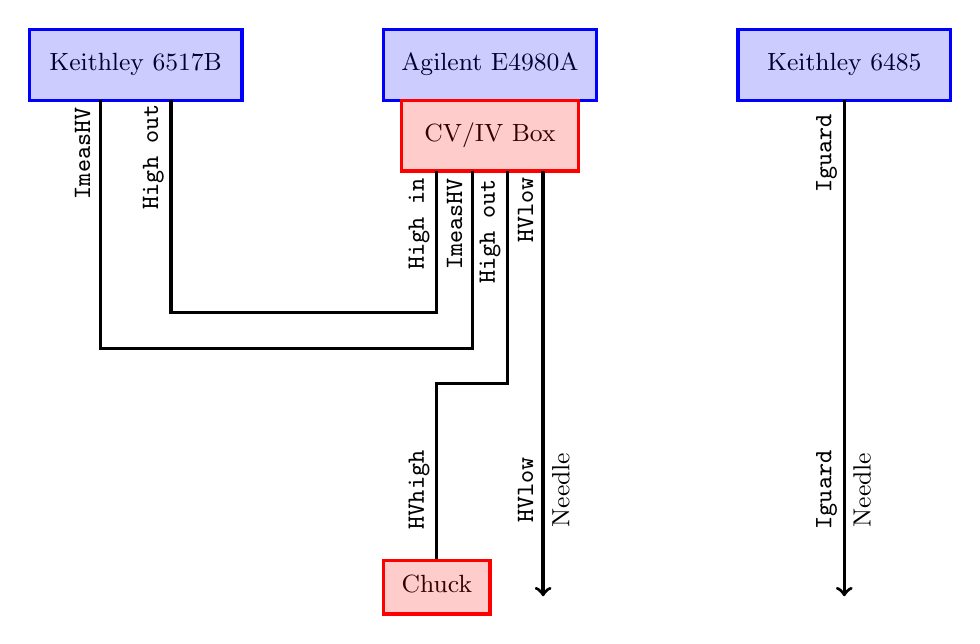
\begin{tikzpicture}
[scale=0.9,blackarrow/.style={->,black,very thick},blueline/.style={->,blue,very thick},redline/.style={->,red,very thick},blackline/.style={black,very thick}]

% Keithley 6517B
\node[->,black](title) at (1.5,0.5,0){\small Keithley 6517B};
\draw[blueline, fill=blue, fill opacity=0.2] (0,0,0) -- (3,0,0) -- (3,1,0) -- (0,1,0) -- cycle;

% Agilent
\node[->,black](title) at (6.5,0.5,0){\small Agilent E4980A};
\draw[blueline, fill=blue, fill opacity=0.2] (5,0,0) -- (8,0,0) -- (8,1,0) -- (5,1,0) -- cycle;

% Keithley 6485
\node[->,black](title) at (11.5,0.5,0){\small Keithley 6485};
\draw[blueline, fill=blue, fill opacity=0.2] (10,0,0) -- (13,0,0) -- (13,1,0) -- (10,1,0) -- cycle;

% cviv box
\node[->,black](title) at (6.5,-0.5,0){\small CV/IV Box};
\draw[redline, fill=red, fill opacity=0.2] (5.25,0,0) -- (7.75,0,0) -- (7.75,-1,0) -- (5.25,-1,0) -- cycle;

% HV out
\draw[blackline] (2,0,0) -- (2,-3,0) -- (5.75,-3,0) -- (5.75,-1,0);
\node[->,black](title) at (1.75,-0.8){\rotatebox{90}{\small {\tt High out}}};
\node[->,black](title) at (5.5,-1.75){\rotatebox{90}{\small {\tt High in}}};

% IV meas
\draw[blackline] (1,0,0) -- (1,-3.5,0) -- (6.25,-3.5,0) -- (6.25,-1,0);
\node[->,black](title) at (0.75,-0.75){\rotatebox{90}{\small {\tt ImeasHV}}};
\node[->,black](title) at (6,-1.75){\rotatebox{90}{\small {\tt ImeasHV}}};

% hi out
\draw[blackline] (6.75,-1.0,0) -- (6.75,-4,0) -- (5.75,-4,0) -- (5.75,-6.5,0);
\node[->,black](title) at (6.5,-1.85){\rotatebox{90}{\small {\tt High out}}};
\node[->,black](title) at (5.5,-5.5){\rotatebox{90}{\small {\tt HVhigh}}};

% chuck
\node[->,black](title) at (5.75,-6.825,0){\small Chuck};
\draw[redline, fill=red, fill opacity=0.2] (5,-6.5,0) -- (6.5,-6.5,0) -- (6.5,-7.25,0) -- (5,-7.25,0) -- cycle;

% lo out
\draw[blackarrow] (7.25,-1.0,0) -- (7.25,-7,0);
\node[->,black](title) at (7,-1.55){\rotatebox{90}{\small {\tt HVlow}}};
\node[->,black](title) at (7,-5.5){\rotatebox{90}{\small {\tt HVlow}}};
\node[->,black](title) at (7.5,-5.5){\rotatebox{90}{\small Needle}};

% gr
\draw[blackarrow] (11.5,0.0,0) -- (11.5,-7,0);
\node[->,black](title) at (11.25,-0.75){\rotatebox{90}{\small {\tt Iguard}}};
\node[->,black](title) at (11.25,-5.5){\rotatebox{90}{\small {\tt Iguard}}};
\node[->,black](title) at (11.75,-5.5){\rotatebox{90}{\small Needle}};

\end{tikzpicture}
\caption[Electrical Connections]{Sketch of the electrical connections.}
\label{fig:electrical}
\end{figure}

The electrical connections between devices are shown in figure~\ref{fig:electrical}.
The triax measurement input of the Keithley 6517B is connected to the {\tt I meas (needle)} connector of the CV/IV box with a BNC cable that is labelled {\tt ImeasHV} on both ends.
The Keithley 6517B's back side HV source output is connected to the {\tt High in (chuck)} connector of the CV/IV box with a red SHV cable labelled {\tt High in (chuck)} on the box side and {\tt High out (chuck)} on the device side.
From the CV/IV box the connector {\tt High out (chuck)} is connected to the chuck, via a red SHV cable marked {\tt High out (chuck)}.
The connector {\tt Low in (needle)} is connected to the {\tt Lo} needle via a BNC cable labelled {\tt HVlow}.
The backside measurement input of the Keithley 6485 is directly connected to the {\tt GR needle}.
The BNC cable is labelled {\tt Iguard} on both ends.\\

\begin{figure}[hbtp!]
\centering
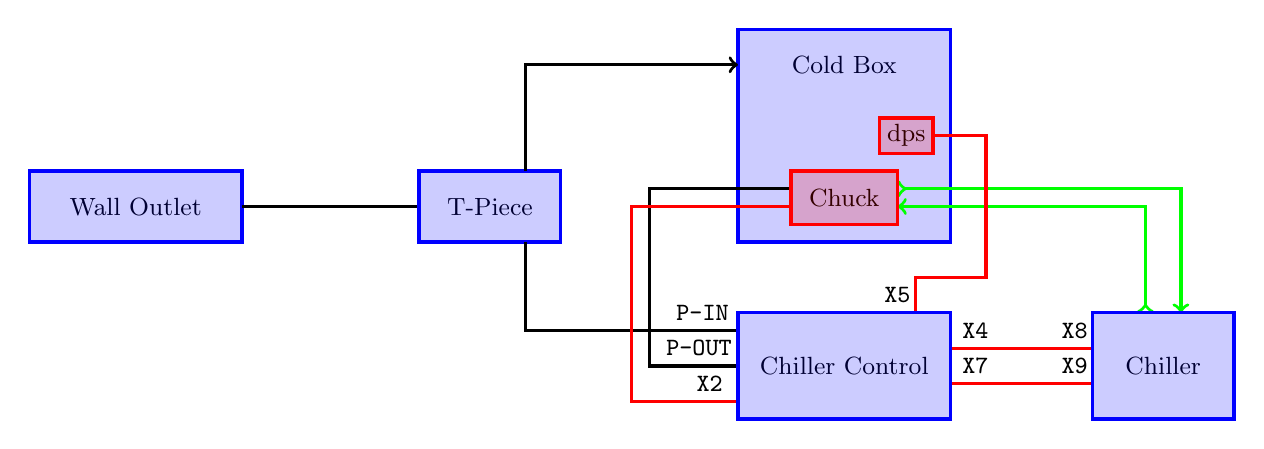
\begin{tikzpicture}
[scale=0.9,blackarrow/.style={->,black,very thick},blueline/.style={->,blue,very thick},redline/.style={red,very thick},blackline/.style={black,very thick},greenline/.style={green,very thick}]

% Wall connector
\node[->,black](title) at (1.5,0.5,0){\small Wall Outlet};
\draw[blueline, fill=blue, fill opacity=0.2] (0,0,0) -- (3,0,0) -- (3,1,0) -- (0,1,0) -- cycle;
\draw[blackline] (3,0.5,0) -- (5.5,0.5,0);

% T-Piece
\node[->,black](title) at (6.5,0.5,0){\small T-Piece};
\draw[blueline, fill=blue, fill opacity=0.2] (5.5,0,0) -- (7.5,0,0) -- (7.5,1,0) -- (5.5,1,0) -- cycle;

% Coldbox
\node[->,black](title) at (11.5,2.5,0){\small Cold Box};
\draw[blueline, fill=blue, fill opacity=0.2] (10,3,0) -- (13,3,0) -- (13,0,0) -- (10,0,0) -- cycle;
\draw[blackarrow] (7,1,0) -- (7,2.5,0) -- (10,2.5,0);

\draw[blackline] (7,0,0) -- (7,-1.25,0) -- (10,-1.25,0);
\node[->,black](title) at (9.5,-1,0){\small {\tt P-IN}};
\node[->,black](title) at (9.45,-1.5,0){\small {\tt P-OUT}};
\draw[blackline] (10,-1.75,0) -- (8.75,-1.75,0) -- (8.75,0.75,0) -- (10.75,0.75,0);
\node[->,black](title) at (9.6,-2,0){\small {\tt X2}};
\draw[redline] (10,-2.25,0) -- (8.5,-2.25,0) -- (8.5,0.5,0) -- (10.75,0.5,0);

\node[->,black](title) at (13.35,-1.25,0){\small {\tt X4}};
\node[->,black](title) at (13.35,-1.75,0){\small {\tt X7}};
\draw[redline] (13,-1.5,0) -- (15,-1.5,0);
\draw[redline] (13,-2,0) -- (15,-2,0);
\node[->,black](title) at (14.75,-1.25,0){\small {\tt X8}};
\node[->,black](title) at (14.75,-1.75,0){\small {\tt X9}};

% coolant
\draw[greenline,>->] (15.75,-1,0) -- (15.75,0.5,0) -- (12.25,0.5,0);
\draw[<-<,greenline] (16.25,-1,0) -- (16.25,0.75,0) -- (12.25,0.75,0);

%dps
\node[->,black](title) at (12.375,1.5,0){\small dps};
\draw[redline, fill=red, fill opacity=0.2] (12,1.25,0) -- (12.75,1.25,0) -- (12.75,1.75,0) -- (12,1.75,0) -- cycle;
\draw[redline] (12.75,1.5,0) -- (13.5,1.5,0) -- (13.5,-0.5,0) -- (12.5,-0.5,0) -- (12.5,-1,0);
\node[->,black](title) at (12.25,-0.75,0){\small {\tt X5}};

% chuck
\node[->,black](title) at (11.5,0.625,0){\small Chuck};
\draw[redline, fill=red, fill opacity=0.2] (10.75,0.25,0) -- (12.25,0.25,0) -- (12.25,1,0) -- (10.75,1,0) -- cycle;

% att control P, X2
\node[->,black](title) at (11.5,-1.75,0){\small Chiller Control};
\draw[blueline, fill=blue, fill opacity=0.2] (10,-2.5,0) -- (13,-2.5,0) -- (13,-1,0) -- (10,-1,0) -- cycle;

% chiller
\node[->,black](title) at (16,-1.75,0){\small Chiller};
\draw[blueline, fill=blue, fill opacity=0.2] (15,-2.5,0) -- (17,-2.5,0) -- (17,-1,0) -- (15,-1,0) -- cycle;

\end{tikzpicture}
\caption[Dry Air and Chiller Connections]{Sketch of the dry air and chiller connections. Dry air piping is shown in in black, electrical connections in red, coolant pipes in green.}
\label{fig:dryair}
\end{figure}

From the dry air outlet on the lab wall next to the door, a hose runs towards the probe station.
It is connected to a t-piece, from which one line goes directly to the cold box, another to the chiller control unit.
From the chiller control unit, a line then goes into the cold box towards the chuck.
Figure~\ref{fig:dryair} shows the default connections.\\

%\afterpage{\null\newpage} % this line might go away...
\newpage

\section{Performing Measurements and Using the Read-Out Software}
\label{sec:meas}

This chapter describes how to do an IV and a CV measurement of a simple diode DUT.
It is assumed that the entire setup is switched off with no active measurement running.
Please make an entry into the setup's log book, stating your name, the date, the measurement you performed and any possible changes you made to the setup.\\

\subsection{General Device Setup}
\label{sec:devicesetup}

Verify that there is no active output from the Keithley 6517B and no ongoing measurement.
You can then open the cold box and, using the microscope, place the DUT on the chuck.
The probe needles should be well out of the way to prevent damage.
With tweezers, gently move the DUT over the outer vacuum hole on the chuck and switch on the vacuum pump to fix the DUT on the chuck.
For a measurement in a dry air atmosphere or for measurements at low temperatures, turn on the dry air flow, as described in section~\ref{sec:chuck}.
If needed, operate the chiller via the touch panel of the control unit and wait for thermal equilibrium.\\

\subsection{Setup for an IV Measurement}
\label{sec:ivsetup}

By operating the probe needles as described in figure~\ref{fig:needle}, carefully place the {\tt HVlow} needle on the DUT surface.
You can then switch on the Keithley 6517B with its switch on the front side of the device.
Set the switch on the CV/IV box to the top (IV) position.
For a simple IV measurement, above steps are sufficient.
To additionally measure the guard ring current, place the {\tt Iguard} needle on the guard ring of the DUT.
You can then switch on the Keithley 6485 with its front-side switch.\\

\subsection{Setup for a CV Measurement}
\label{sec:cvsetup}

For a CV measurement, turn on the Agilent E4980A with its front-side switch and wait for it to warm up.
Before connecting any probe needles, you should perform an open measurement for calibration.
To do this, press the {\tt Meas Setup} button on the front of the device\footnote{If the device does not react to the buttons, verify that no read-out software is running. If the Agilent E4980A is being accessed via USB or GPIB, the control buttons are deactivated.}.
With the keys on the right of the display, select {\tt Correction} and then {\tt Meas Open}.
After a successful calibration, you can place the {\tt HVlow} needle on the DUT surface.
Press the button {\tt Display Format} to return to the main screen.
You can then switch on the Keithley 6517B.
The Keithley 6485 is not needed for a CV measurement and can remain switched off.\\

\subsection{Performing a Measurement}
\label{sec:ivmeas}

Log in to the read-out computer with your user credentials.
Navigate to

\medskip
\begin{lstlisting}
D:\Probestation
\end{lstlisting}
\medskip

and run the software by double-clicking on the link {\tt Probestation}.
This will execute the command

\medskip
\begin{lstlisting}
C:\Programfiles\Anaconda3\python.exe gui.py D:\Measurements
\end{lstlisting}
\medskip

in that folder.
The software GUI will start with the IV tab open, as shown in figure~\ref{fig:softwareopeniv}.\\

For an IV measurement, select the starting voltage and the end voltage in the respective fields.
Both positive and negative numbers are accepted.
The field {\tt Abs step} is used to select the absolute value of each step of the voltage ramp.\\

The following field, {\tt Abs compliance current}, should be set to the software compliance limit for this measurement.
If the absolute value of the current measured by the Keithley 6517B exceeds this value, the voltage source will immediately switch the output off and ramp the voltage down to $0\,\volt$.
The following check box enables a guard ring measurement with the Keithley 6485, which of course has to be switched on for this.
If activated, the Keithley 6485 will also check for current compliance and, if reached, turn the Keithley 6517B's voltage output off.
{\tt Wait time} specifies the time in seconds the Keithley 6517B waits before incrementing the voltage output in a ramp.\\

The final field allows the user to select a folder in which the measurement results will be saved.
It defaults to the first command-line argument.
All measurements are saved with the file name corresponding to date and time of the begin of the measurement.\\

The CV tab shown in figure~\ref{fig:softwareopencv} looks similar, with the difference that the fields for current compliance and guard ring measurement are substituted by fields where the frequency parameters can be set.
The first one sets the measurement frequency of the Agilent E4980A, the {\tt AC Voltage level} field sets the AC voltage.\\

{\bf Beware that in CV and Strip measurements, there is no software current compliance!}\footnote{This is because the large internal resistance of the Agilent E4980A and the CV/IV box distorts the current measurement of the Keithley 6517B.}\\

You should therefore first do an IV measurement to verify that your desired voltage range is safe for your DUT.\\

\begin{figure}[hbtp]
\centering
\begin{subfigure}[t]{0.475\textwidth}
\centering\captionsetup{width=.8\linewidth}%
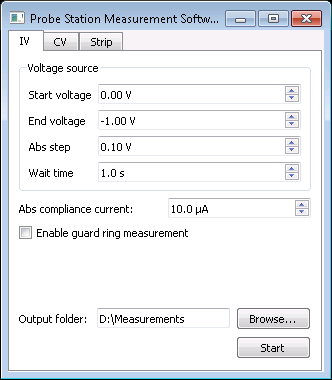
\includegraphics[width=\linewidth]{pictures/softiv.png}
\caption[Software with the IV Tab]{Initial window of the measurement software, with the IV tab open.}
\label{fig:softwareopeniv}
\end{subfigure}
\begin{subfigure}[t]{0.475\textwidth}
\centering\captionsetup{width=.8\linewidth}%
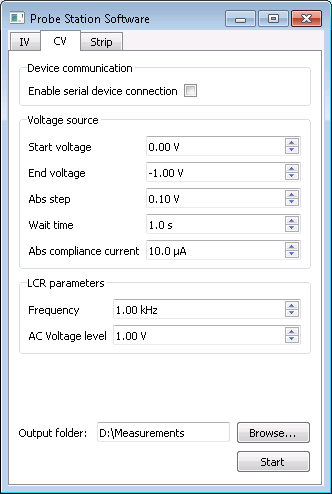
\includegraphics[width=\linewidth]{pictures/softcv.png}
\caption[Software with the CV Tab]{The measurement software with the CV tab selected.}
\label{fig:softwareopencv}
\end{subfigure}
\end{figure}

For both measurement types, clicking on {\tt Start} begins the measurement.
A new window will open with a live display of the measurements.
An example ongoing IV measurement with guard ring current measurement is shown in figure~\ref{fig:ivmeas}, a running CV measurement in figure~\ref{fig:cvmeas}.\\

\begin{figure}[hbtp]
\centering
\begin{subfigure}[t]{0.475\textwidth}
\centering\captionsetup{width=.8\linewidth}%
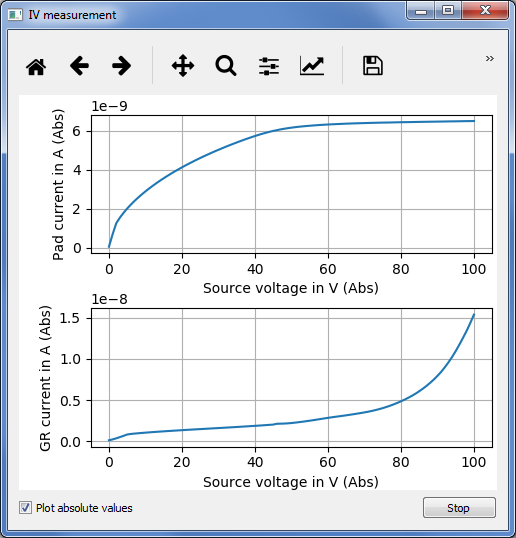
\includegraphics[width=\linewidth]{pictures/ivmeas.png}
\caption[Running IV Measurement]{Ongoing IV measurement. The top plot shows the IV characteristic, the bottom plot the guard ring current.}
\label{fig:ivmeas}
\end{subfigure}
\begin{subfigure}[t]{0.475\textwidth}
\centering\captionsetup{width=.8\linewidth}%
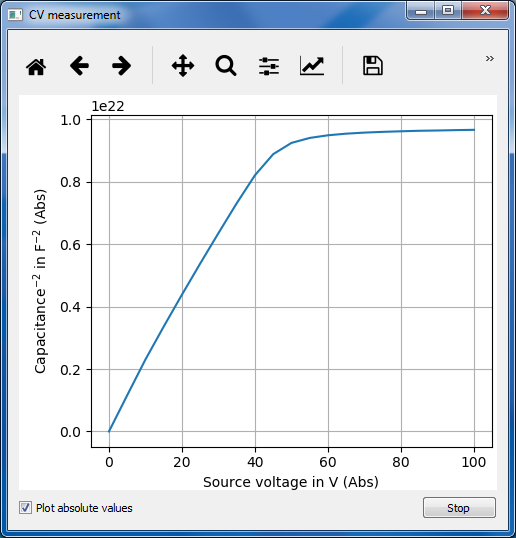
\includegraphics[width=\linewidth]{pictures/cvmeas.png}
\caption[Running CV Measurement]{Ongoing CV measurement. The y-axis shows the inverse square of the measured capacitance.}
\label{fig:cvmeas}
\end{subfigure}
\end{figure}

In both measurement windows, there is a button to show the absolute measurement values.
Clicking the {\tt Stop} button will ramp down the output voltage to $0\,\volt$ and switch the output off.
This will also happen if the measurement window is closed or should crash.
If an IV with guard ring measurement is selected, the bottom plot will show the guard ring current.
In a CV measurement, the inverse square of the measured capacitance is displayed.\\

On reaching the specified end voltage, the voltage will be ramped down to $0\,\volt$.
After finishing your measurements, close the software and switch off the Keithley 6517B and 6485 and the Agilent E4980A.
If you used the chiller, set the temperature to room temperature and wait for thermal equilibrium.
Then switch off the chiller control unit and then the chiller via the large red switch.
After verifying that there is no voltage output, you can open the cold box and, using the microscope, detach the probe needles.
Then switch the vacuum off and carefully remove your DUT before closing the cold box.\\

\subsection{Installing the Software}
\label{sec:installation}

The software has been tested to run on Ubuntu 18.04, Raspbian Stretch, CERN CentOS 7 and Microsoft Windows 7.
It is already preinstalled on {\tt fhlprobest.desy.de}.

\subsubsection{Ubuntu 18.04}

\paragraph{Normal Installation\\}
On Ubuntu 18.04 you first have to install {\tt git} and {\tt pip} for python

\medskip
\begin{lstlisting}
sudo apt-get install git python3-pip
\end{lstlisting}
\medskip

Then upgrade {\tt pip} to the latest version

\medskip
\begin{lstlisting}
sudo pip3 install --upgrade pip
\end{lstlisting}
\medskip

You can then install the required python packages

\medskip
\begin{lstlisting}
sudo pip3 install pyvisa pyvisa-py numpy matplotlib pyserial pyqt5
\end{lstlisting}
\medskip

For a serial connection, your user account has to be added to the {\tt dialout} group

\medskip
\begin{lstlisting}
sudo usermod -a -G dialout $USER
\end{lstlisting}
\medskip

Then download the repository with

\medskip
\begin{lstlisting}
git clone https://github.com/thomaseichhorn/probestation.git /where/you/want/to/install
\end{lstlisting}
\medskip

After logging off and logging in again to refresh the user permissions, you should be able to run the software from the directory you specified before with the command

\medskip
\begin{lstlisting}
python3 gui.py
\end{lstlisting}
\medskip

\paragraph{Advanced Options\\}
These commands should not be needed, but are listed here as reference.

\begin{itemize}
\item{} If you do not have {\tt sudo} rights, append a {\tt -{}-user} to the {\tt pip3} commands to install the python packages for your user only.

\item{} To use {\tt Python 2.7}, run {\tt sudo apt-get install python-pip} to get {\tt pip2}.
Then install the python packages, substituting {\tt pip2} for {\tt pip3} and run the program with the command {\tt python gui.py}.

\item{} The program automatically defaults back to {\tt Qt4} if {\tt Qt5} can not be found.
The {\tt Qt4} packages can't be installed by {\tt pip}, but have to be installed with {\tt sudo apt-get install python-qt4} for {\tt Python 2.7} and {\tt sudo apt-get install python3-pyqt4} for {\tt Python 3}.
\end{itemize}

\subsubsection{Raspbian Stretch}

Currently, {\tt Qt5} is not available via the package manager, so the easiest way to run the software is with {\tt Python 2} using {\tt Qt 4}.
You will need to install some packages

\medskip
\begin{lstlisting}
sudo apt-get install git python-qt4
\end{lstlisting}
\medskip

Upgrade {\tt pip} to the latest version with

\medskip
\begin{lstlisting}
sudo pip install --upgrade pip
\end{lstlisting}
\medskip

You can then install the required python packages

\medskip
\begin{lstlisting}
sudo pip install pyvisa pyvisa-py numpy matplotlib pyserial
\end{lstlisting}
\medskip

For a serial connection, your user account has to be added to the {\tt dialout} group

\medskip
\begin{lstlisting}
sudo usermod -a -G dialout $USER
\end{lstlisting}
\medskip

Then download the repository with

\medskip
\begin{lstlisting}
git clone https://github.com/thomaseichhorn/probestation.git /where/you/want/to/install
\end{lstlisting}
\medskip

After logging off and logging in again to refresh the user permissions, you should be able to run the software from the directory you specified before with the command

\medskip
\begin{lstlisting}
python gui.py
\end{lstlisting}
\medskip

\subsubsection{CERN CentOS 7}

On CERN CentOS 7 you also first have to install {\tt git} and {\tt python3}.
Open a root terminal and run

\medskip
\begin{lstlisting}
yum install centos-release-scl
\end{lstlisting}
\medskip

to enable software collections and then run

\medskip
\begin{lstlisting}
yum install rh-python35 git
\end{lstlisting}
\medskip

Then you can load the {\tt python3} environment

\medskip
\begin{lstlisting}
source /opt/rh/rh-python35/enable
\end{lstlisting}
\medskip

and upgrade {\tt pip} to the latest version

\medskip
\begin{lstlisting}
pip3 install --upgrade pip
\end{lstlisting}
\medskip

You can then install the required python packages

\medskip
\begin{lstlisting}
pip3 install pyvisa pyvisa-py numpy matplotlib pyserial pyqt5
\end{lstlisting}
\medskip

For a serial connection, your user account has to be added to the dialout group

\medskip
\begin{lstlisting}
usermod -a -G dialout <yourusername>
\end{lstlisting}
\medskip

You can now close the root terminal.
Then download the repository with

\medskip
\begin{lstlisting}
git clone https://github.com/thomaseichhorn/probestation.git /where/you/want/to/install
\end{lstlisting}
\medskip

After logging off and logging in again to refresh the user permissions, load the {\tt python3} environment again

\medskip
\begin{lstlisting}
source /opt/rh/rh-python35/enable
\end{lstlisting}
\medskip

You should be able to run the software from the directory you specified before with the command

\medskip
\begin{lstlisting}
python3 gui.py
\end{lstlisting}
\medskip

\subsubsection{Microsoft Windows 7}

On Microsoft Windows 7 you need a Python environment, such as {\tt Miniconda}\footnote{\href{https://conda.io/miniconda.html}{https://conda.io/miniconda.html}}.
If you have a DESY Windows installation, use DSM to install {\tt Anaconda} (Software Categories $\rightarrow$ Programming).
With the {\tt Anaconda prompt} (or from the Windows command line) you can install the needed python packages with the command

\medskip
\begin{lstlisting}
conda install -c conda-forge pyvisa pyvisa-py numpy matplotlib pyserial pyqt
\end{lstlisting}
\medskip

Otherwise you can select these packages with the Anaconda Navigator.
Assuming you downloaded the software to {\tt C:\textbackslash some\textbackslash directory}, you can then run the software with

\medskip
\begin{lstlisting}
python C:\some\directory\gui.py
\end{lstlisting}
\medskip

from the {\tt Anaconda prompt} or from the Windows command line.

\subsection{Recompiling the User Manual}

To recompile the user manual, you need a working latex installation with some additional packages.

\subsubsection{Ubuntu 18.04 and Raspbian Stretch}

On Ubuntu 18.04 and Raspbian Stretch you need to install several {\tt latex} packages via

\medskip
\begin{lstlisting}
sudo apt-get install texlive-latex-base texlive-science texlive-latex-extra
\end{lstlisting}
\medskip

You can then build the documentation with the command

\medskip
\begin{lstlisting}
cd doc && pdflatex manual.tex
\end{lstlisting}
\medskip

\subsubsection{CERN CentOS 7}

On CERN CentOS 7 you will need to install several {\tt latex} packages.
Unfortunately, the easiest way is to install all available ones from a root terminal

\medskip
\begin{lstlisting}
yum install texlive-*
\end{lstlisting}
\medskip

You then have to download some packages manually

\medskip
\begin{lstlisting}
cd doc
wget http://www.cs.cmu.edu/afs/cs/misc/tex/common/teTeX-1.0/lib/texmf/tex/latex/misc/SIunits.sty
wget http://www.cs.cmu.edu/afs/cs/misc/tex/common/teTeX-1.0/lib/texmf/tex/latex/misc/tocbibind.sty
wget http://www.cs.cmu.edu/afs/cs/misc/tex/common/teTeX-1.0/lib/texmf/tex/latex/misc/stdclsdv.sty
\end{lstlisting}
\medskip

Before you can then build the documentation

\medskip
\begin{lstlisting}
pdflatex manual.tex
\end{lstlisting}
\medskip

\subsubsection{Microsoft Windows 7}

This is beyond the scope of this document, there are good step-by-step instructions on the internet.

\newpage
\begin{thebibliography}{}

\bibitem{ref:github} Thomas Eichhorn and Jonas R\"ubenach.\\ {\em Probe Station Manual and Software}.\\ \href{https://github.com/thomaseichhorn/probestation}{https://github.com/thomaseichhorn/probestation}\\ Link accessed 09.04.2018.

\bibitem{ref:keithley6517bref} Keithley Instruments, Inc.\\ {\em Model 6517B Electrometer User’s Manual}.\\ \href{http://download.tek.com/manual/6517B-900-01--A-Jun2008--User.pdf}{http://download.tek.com/manual/6517B-900-01--A-Jun2008--User.pdf}\\ Link accessed 27.03.2018.

\bibitem{ref:agilentref} Keysight Technologies\\ {\em Keysight E4980A/AL Precision LCR Meter}.\\ \href{https://literature.cdn.keysight.com/litweb/pdf/E4980-90220.pdf?id=789356}{https://literature.cdn.keysight.com/litweb/pdf/E4980-90220.pdf?id=789356}\\ Link accessed 27.03.2018.

\bibitem{ref:keithley6485ref} Keithley Instruments, Inc.\\ {\em Model 6485 Picoammeter Instruction Manual}.\\ \href{http://download.tek.com/manual/6485-901-01(A-Nov2001)(Instruction).pdf}{http://download.tek.com/manual/6485-901-01(A-Nov2001)(Instruction).pdf}\\ Link accessed 27.03.2018.

\end{thebibliography}

\end{document}
